\documentclass[12pt]{article}
  \usepackage{graphicx}
  \usepackage[font=small,labelfont=bf]{caption}
  \usepackage{xcolor,colortbl, wrapfig}
  \usepackage{float}
  \usepackage{array}
  \graphicspath{{images/}}

\pagestyle{empty}
\setcounter{secnumdepth}{2}
\newcolumntype{a}{>{\columncolor{Gray}}c}
\newcolumntype{b}{>{\columncolor{white}}c}

\usepackage{titlesec}

\topmargin=0cm
\oddsidemargin=0cm
\textheight=22.0cm
\textwidth=16cm
\parindent=0cm
\parskip=0.15cm
\topskip=0truecm
\raggedbottom
\abovedisplayskip=3mm
\belowdisplayskip=3mm
\abovedisplayshortskip=0mm
\belowdisplayshortskip=2mm
\normalbaselineskip=12pt
\normalbaselines

\begin{document}

\vspace*{0.5in}
\centerline{\bf\Large Design Document}

\vspace*{0.5in}
\centerline{\bf\Large Team PB-PJ}

\vspace*{0.5in}
\centerline{\bf\Large 18 March 2018}

\vspace*{1.5in}
\begin{table}[htbp]
\caption{Team PB-PJ}
\begin{center}
\begin{tabular}{|r | c|}
\hline
Name\\
\hline\hline
Matthew Ferderber\\
Matthew Dugal\\
Mylene Haurie\\
Viktoriya Malinova\\
Eric Morgan\\
Artem Khomich\\
Kai Nicoll-Griffith\\
Maxmilien Malderle\\
\hline
\end{tabular}
\end{center}
\end{table}

\clearpage

\section{Introduction}

The design document provides a detailed view into the design of the application
and justifies the various design decisions made by the programmers. The architecture design section
provides a high-level view of the architectural choices while the detailed design section
focuses on the detailed implementation of the architecture and all aspects of the system.
The Subsystem Interface Specification describes the two major Subsystems of the
application and all of their components.

\section{Architectural Design} \label{sec:arch}

The My Money application uses the Model View Controller architecture to seperate code into
logical components (models, view, and controllers).

\subsubsection{Models}

Models are used to provide a simple interface for the data used by the application uses.
Whenever changes are made in the model (by the controller), the view is notified and updated.

\subsubsection{Views}

Views are the visual representation of the models. Any data that needs to be shown to the user is
given to the view through models and is updated when changes are made to the model.
The view can also be updated by the controller. When an action is performed by the user,
the view delivers the action to the controller which provides the logic behind the requested
action.

\subsubsection{Controllers}

Controllers provide the logic that allows for interaction between the user and the application.
When an action is performed by the user it is relayed from the view to the responsible controller.
The controller uses its internal state to decide what the outcome of the action should be.
When the outcome is decided, the controller can update which view the application displays
or the model that is bound to the current view.

\subsubsection{Benefits}

MVC provides many benefits for the application. It allows for seperation of display, logic and 
data access into components. Because components are seperated, the same portions of the project
can be worked on by multiple people in parallel. Without having to worry about the status of the whole
application, a view can be updated to display data differently, 
the model can be modified to contain more data, and the controller can
handle new actions.


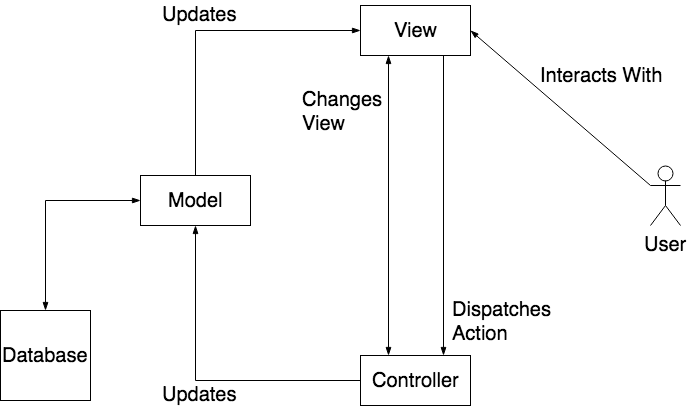
\includegraphics[scale=0.7]{archdesigndiagram}\\

This diagram shows the interaction between the models, views, and controllers.
As described above, the user interacts with the view which displays data from the model.
The view can send actions to the controller which prompts an update of the view/model.
The model (and Data Access Objects) interact with the database to update and retrieve data.

\subsection{Architectural Diagram}
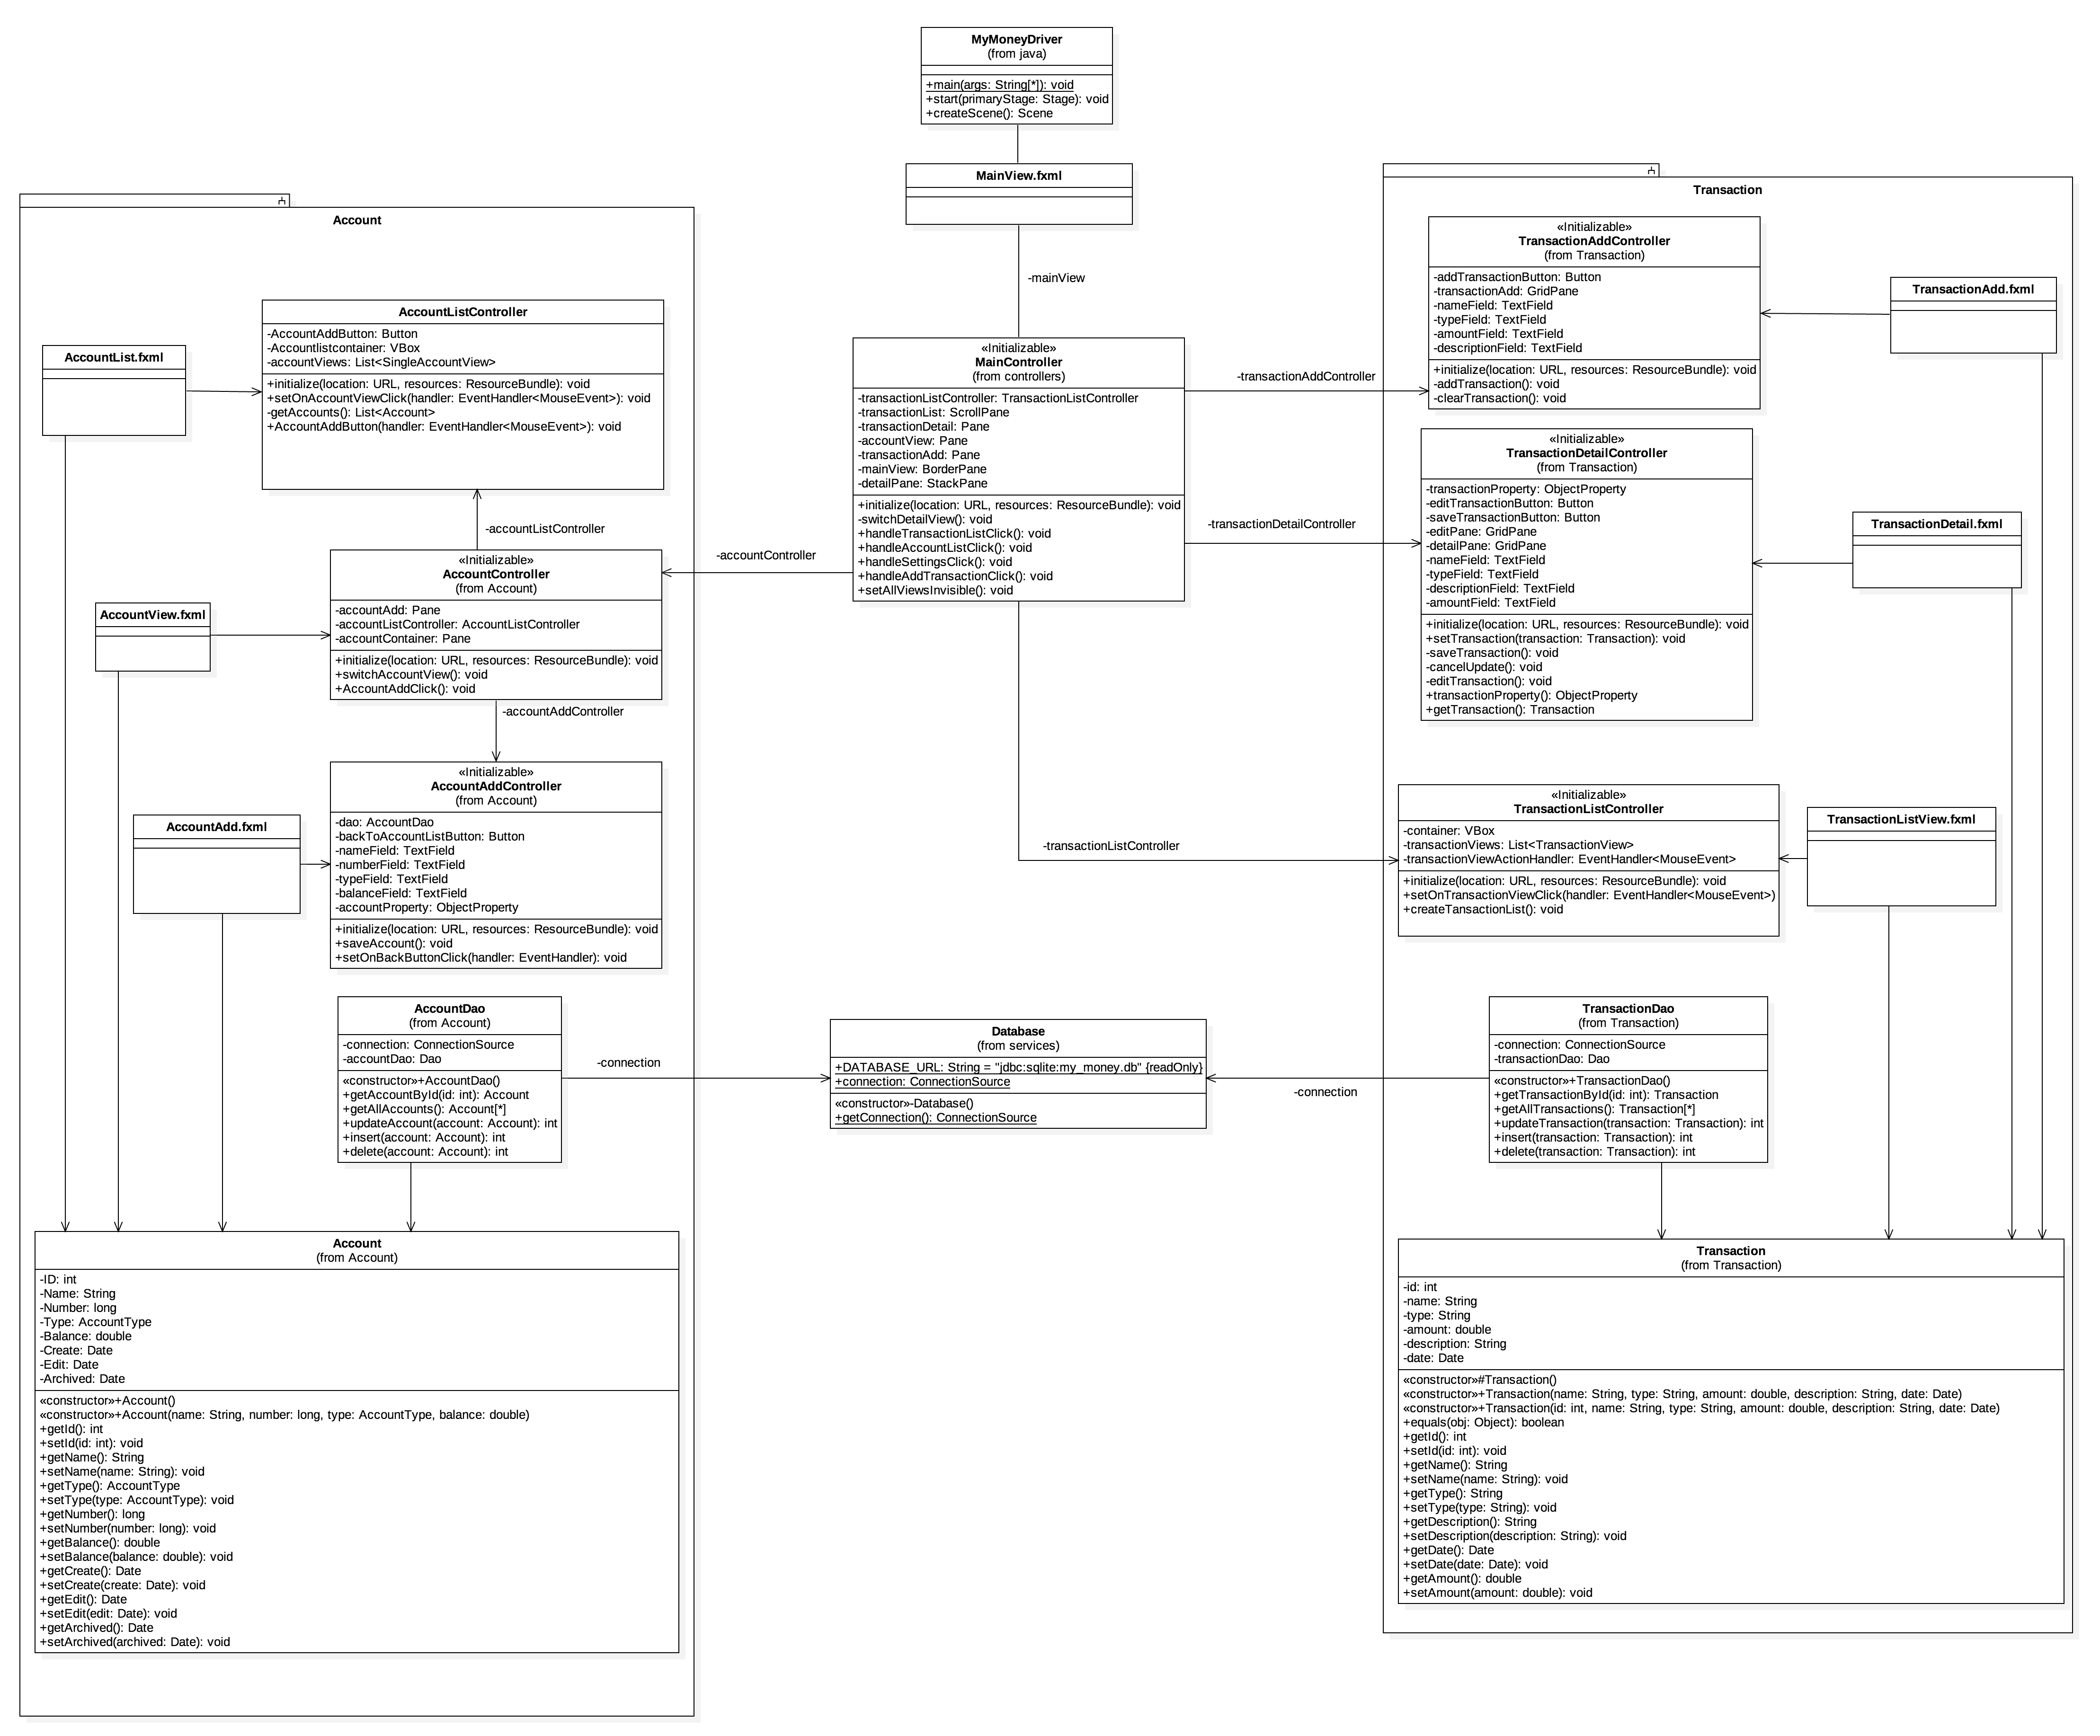
\includegraphics[scale=0.12]{classdiagram}

The MVC architecture of the system allows for the project to be modularized
into multiple submodules. This diagram shows the Account and Transaction
submodules which make up the main functionality of the system. Organizing the system
like this allows for major re-use of components such as the models (Account and Transaction)
which are used for every view in their respective module.

\subsection{Subsystem Interface Specifications}

\subsubsection{Account Subsystem Interface}

The Account Subsystem is the system that allows the user to manage
their accounts used to store transactions. Accounts are typically used
to represent real bank accounts or similar real-world accounts that transactions
can take place with. There are three main
views associated with the account system. The detailed view, list view, and add view.

\subsubsection{Account List View}

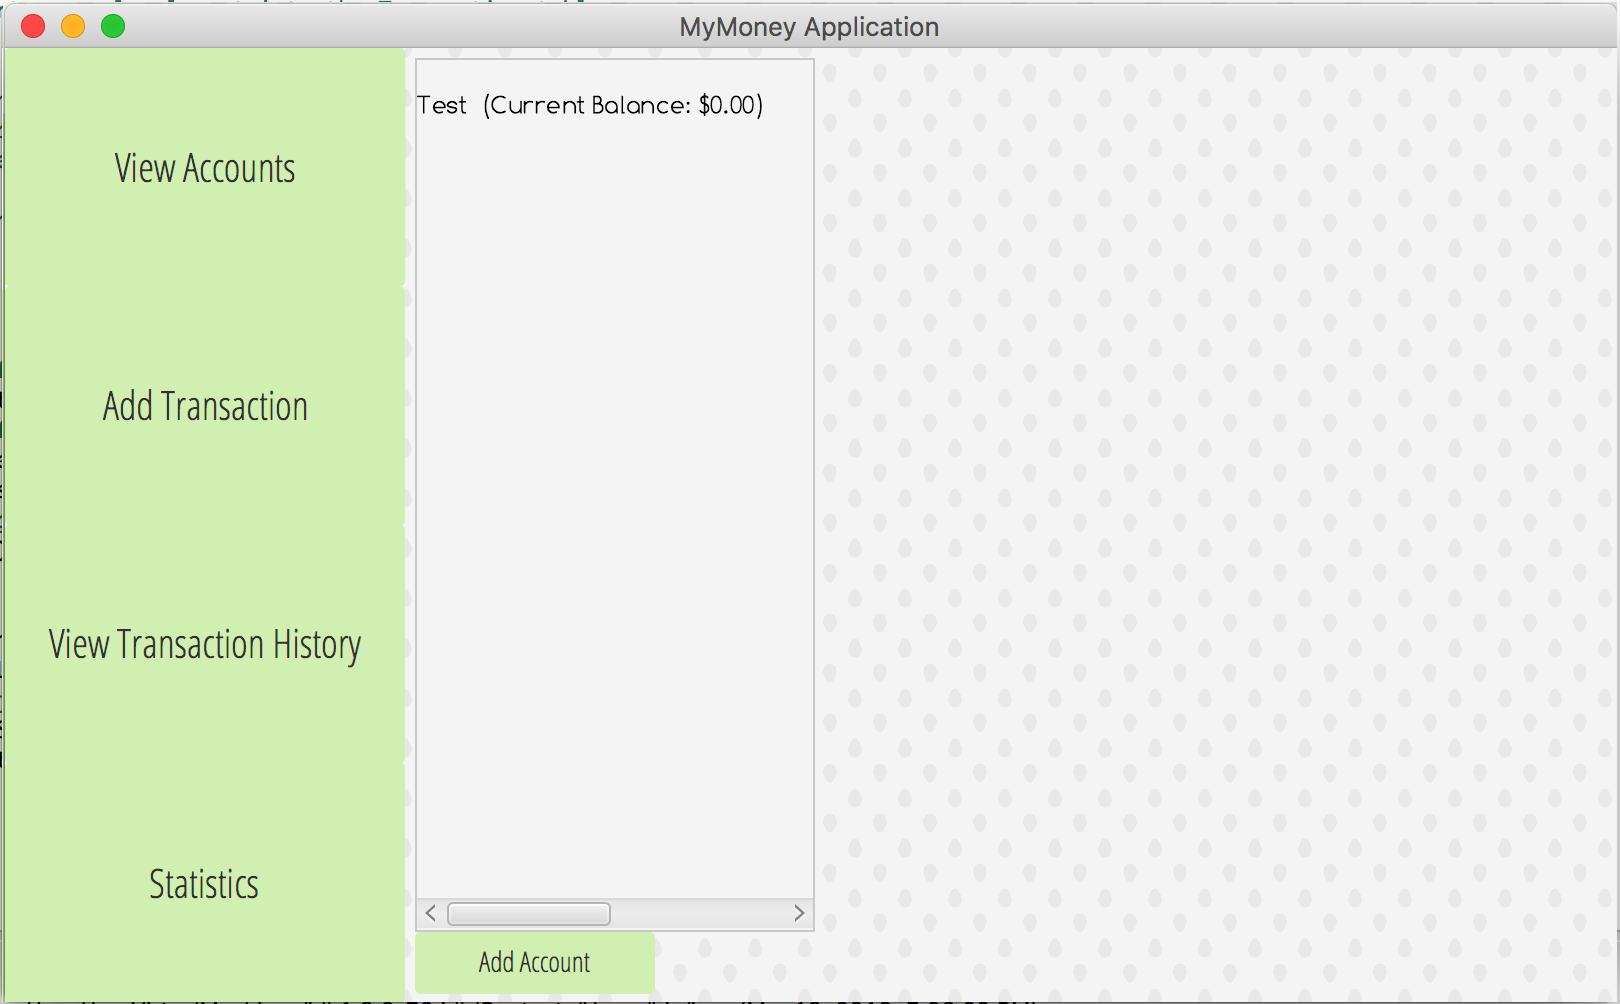
\includegraphics[scale=0.2]{accountlist}

The Account list is responsible for showing an up-to-date list of all of
the accounts in the application. From the Account List, the user can enter
into the Detailed view and the Add view by double clicking on a list item
or clicking on the add Account button respectively.\\

The AccountListController is used to manage switching between
views related to the Account List (as seen in the class diagram). 
The AccountListController will either call the 
``AccountViewActionHandler'' or the ``AccountAddClick'' event handlers
when the view is interacted with by the user.


\subsubsection{Account Detailed View}

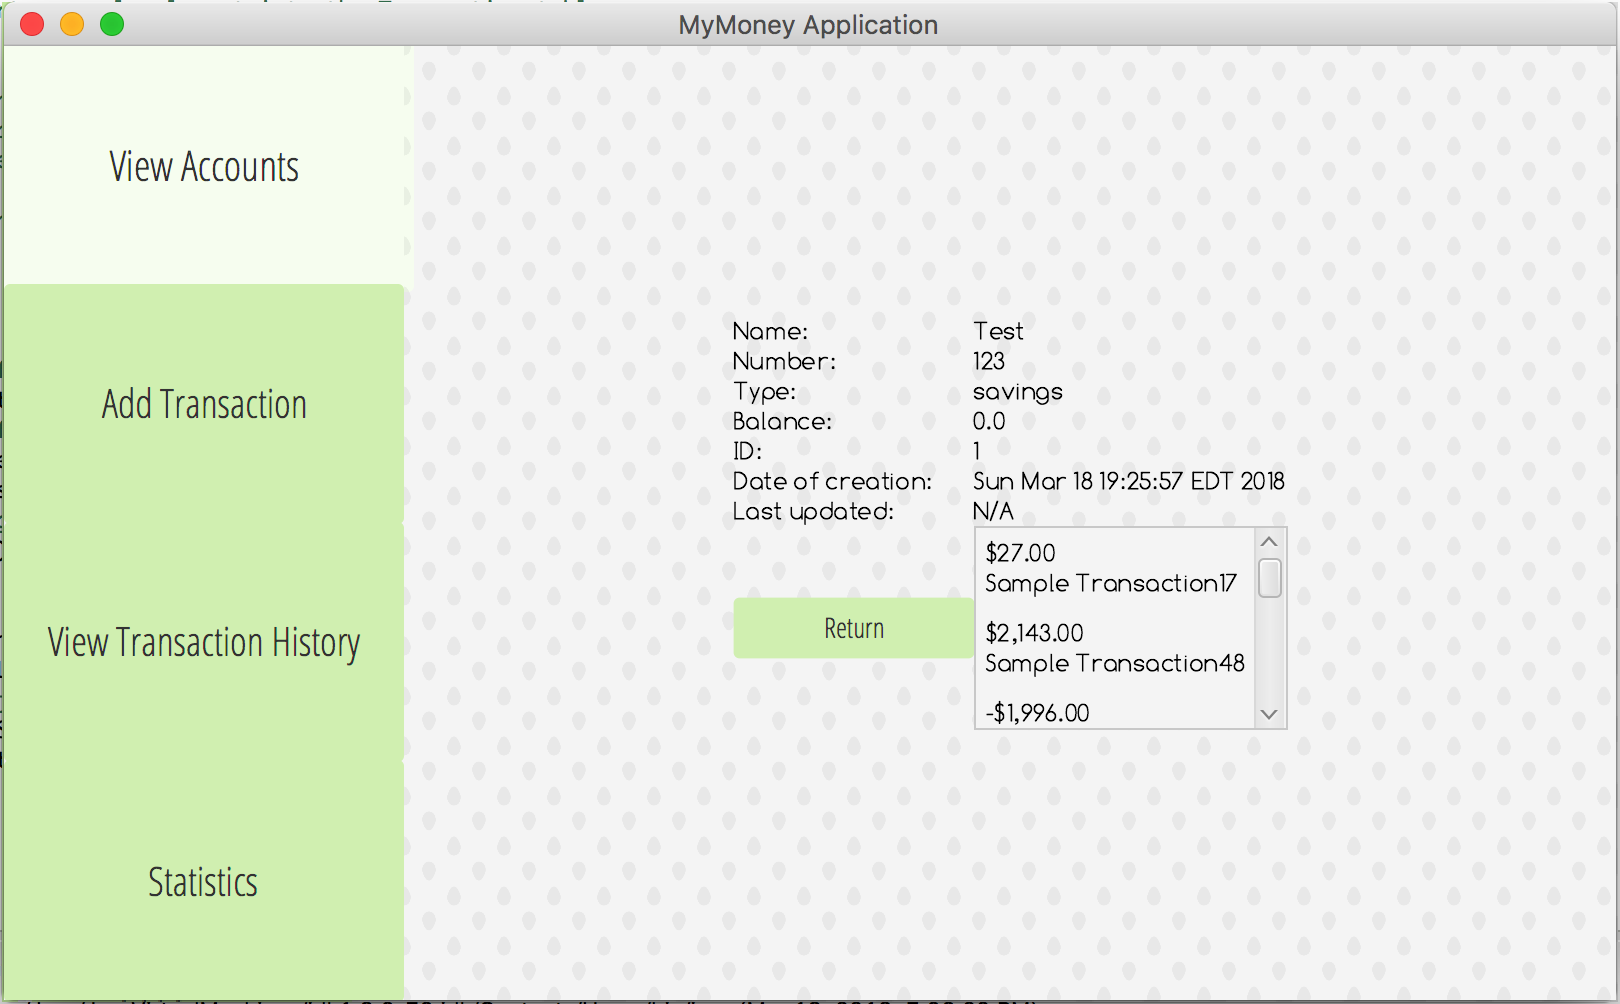
\includegraphics[scale=0.2]{accountdetail}

The Detailed view represents one Account and is responsible for
showing all of the details associated with the selected account. 
Due to the informational nature of the detail view, there are no actions
the user can perform in the view.

\subsubsection{Account Add View}

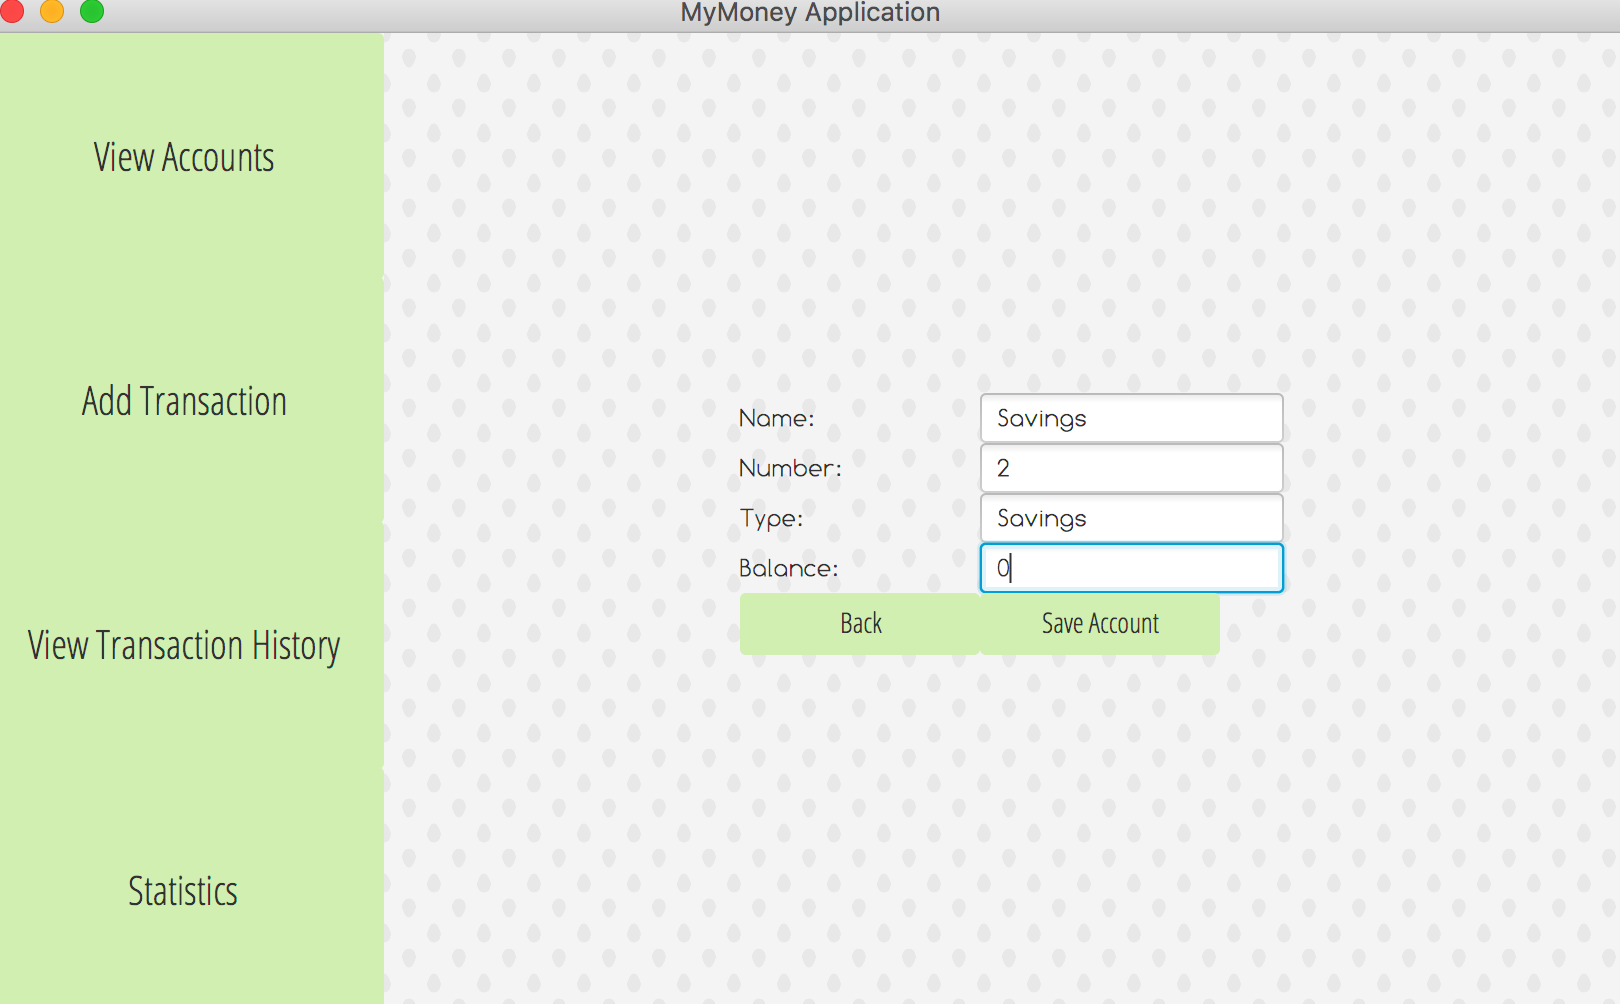
\includegraphics[scale=0.2]{accountadd}

The Account Add view is used for creating new accounts in the system.
When creating an account, the user enters the relevant account details
(Account name, number, account type, and initial balance).\\

When the user saves the account, the AccountAddController is passed the
action by the AccountAddView. The ``saveAccount'' method is called
which retrieves the new accounts details from the view and inserts it into the
database using the AccountDAO. Once inserted, the user is returned to the
Account List view where they can continue interacting with the system.

\subsubsection{Transaction Subsystem Interface}

The Transaction Subsystem allows the user to add, delete, and edit
transactions associated with an account. Transactions represent real-world
currency transactions and have a Name, type, amount, description, and 
associated account. Transactions have three main views. The Transaction list view,
detail view, and add view.

\subsubsection{Transaction List View}

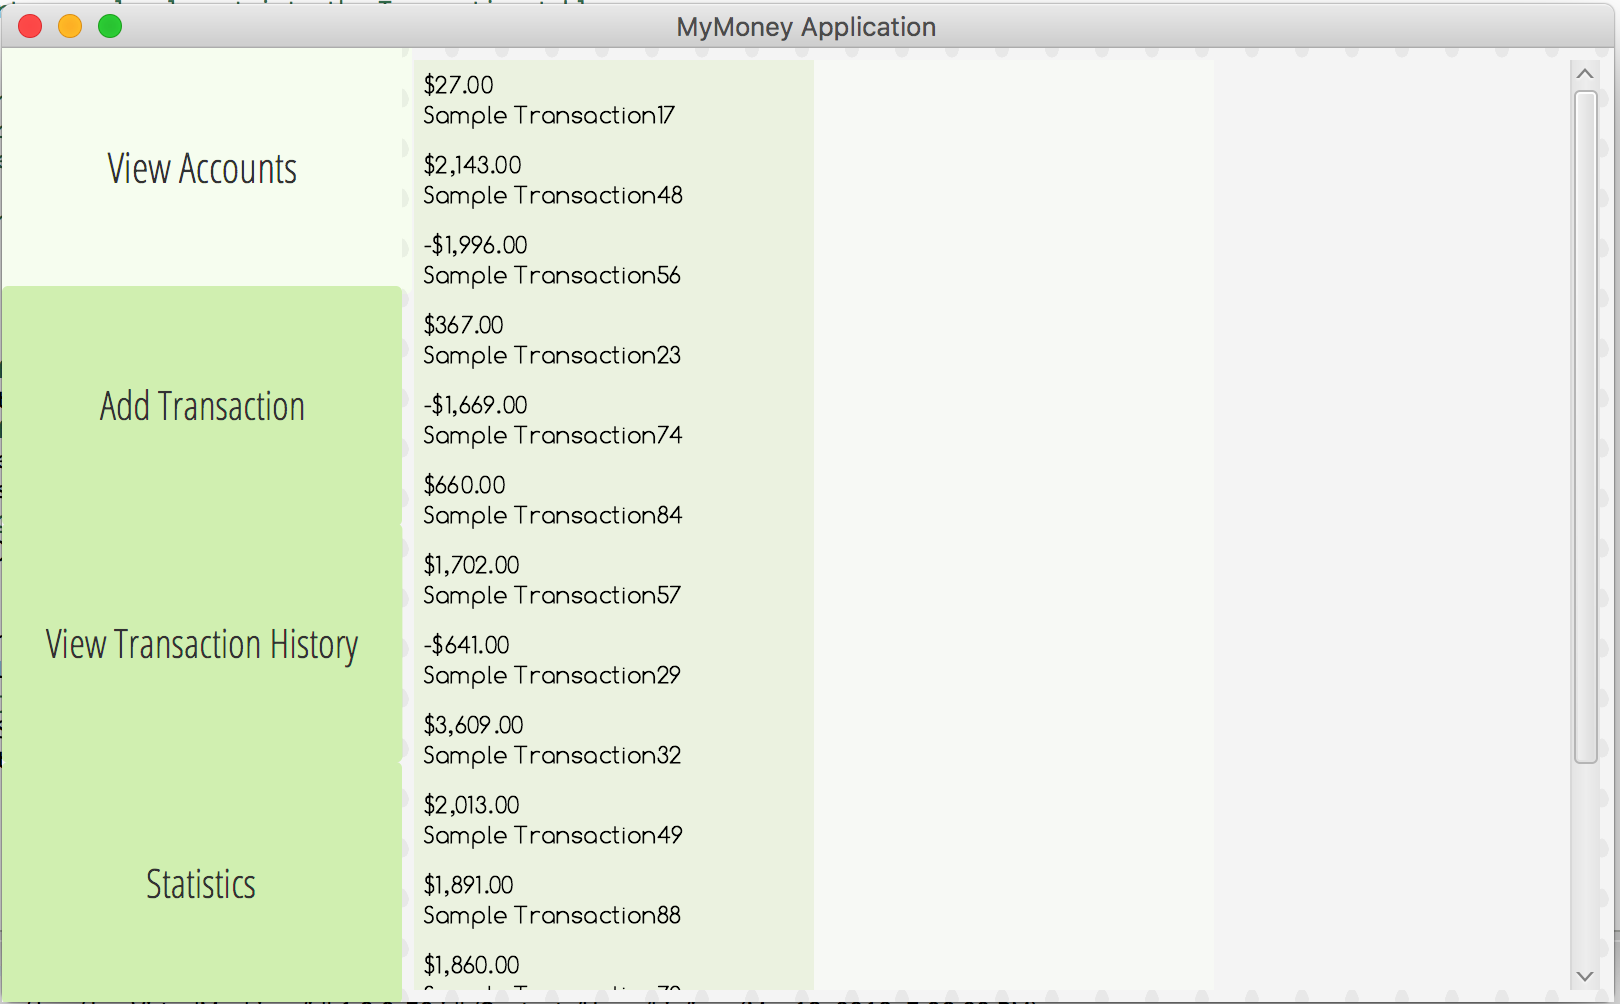
\includegraphics[scale=0.2]{transactionlist}

The Transaction List is used to show all of the transactions and a brief
description of what they represent (amount and name). The list is
expandable using the scroll wheel which allows the user to view all of
their transactions sorted by date in descending order.\\

From the Transaction List, the user can click on any transaction to be
brought to the Detailed Transaction View. When a transaction is clicked,
the event handler passed to the TransactionListController by the MainController
is executed which the main view uses to decide which transaction to create in the
TransactionDetail. In this way, the MainController acts as a dispatcher which takes
events and handles the high-level event of displaying different views.

\subsubsection{Transaction Detail View}
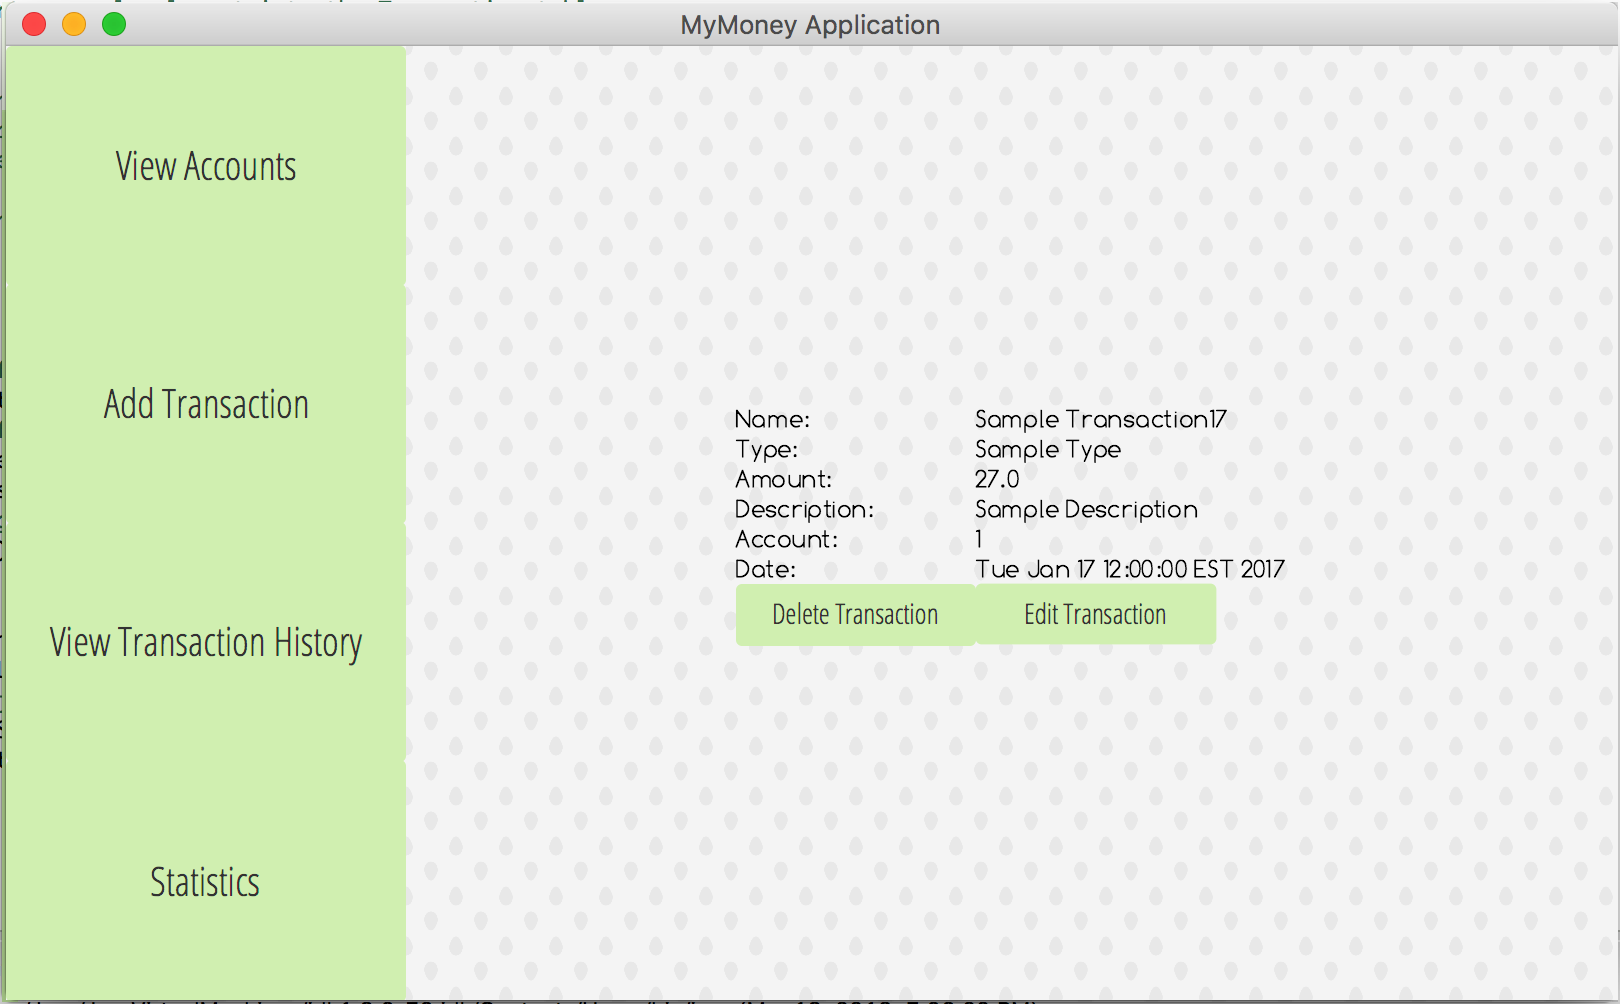
\includegraphics[scale=0.2]{transactiondetail}

The Transaction Detail view displays a full description of the selected
transaction. From this view, the user can see the creation date, and all of the
original data from the creation of the transaction.\\

From the Transaction Detail, the user has two actions: Delete and Edit.
When the user presses delete, the TransactionDetailController's ``deleteTransaction'' method
is called and the transaction is deleted. Once deleted, the user is returned to
the Transaction List view. When the Edit action is invoked, the
TransactionDetailController's ``editTransaction'' method is called which
changes the view to allow all fields to be edited.

\subsubsection{Transaction Add View}

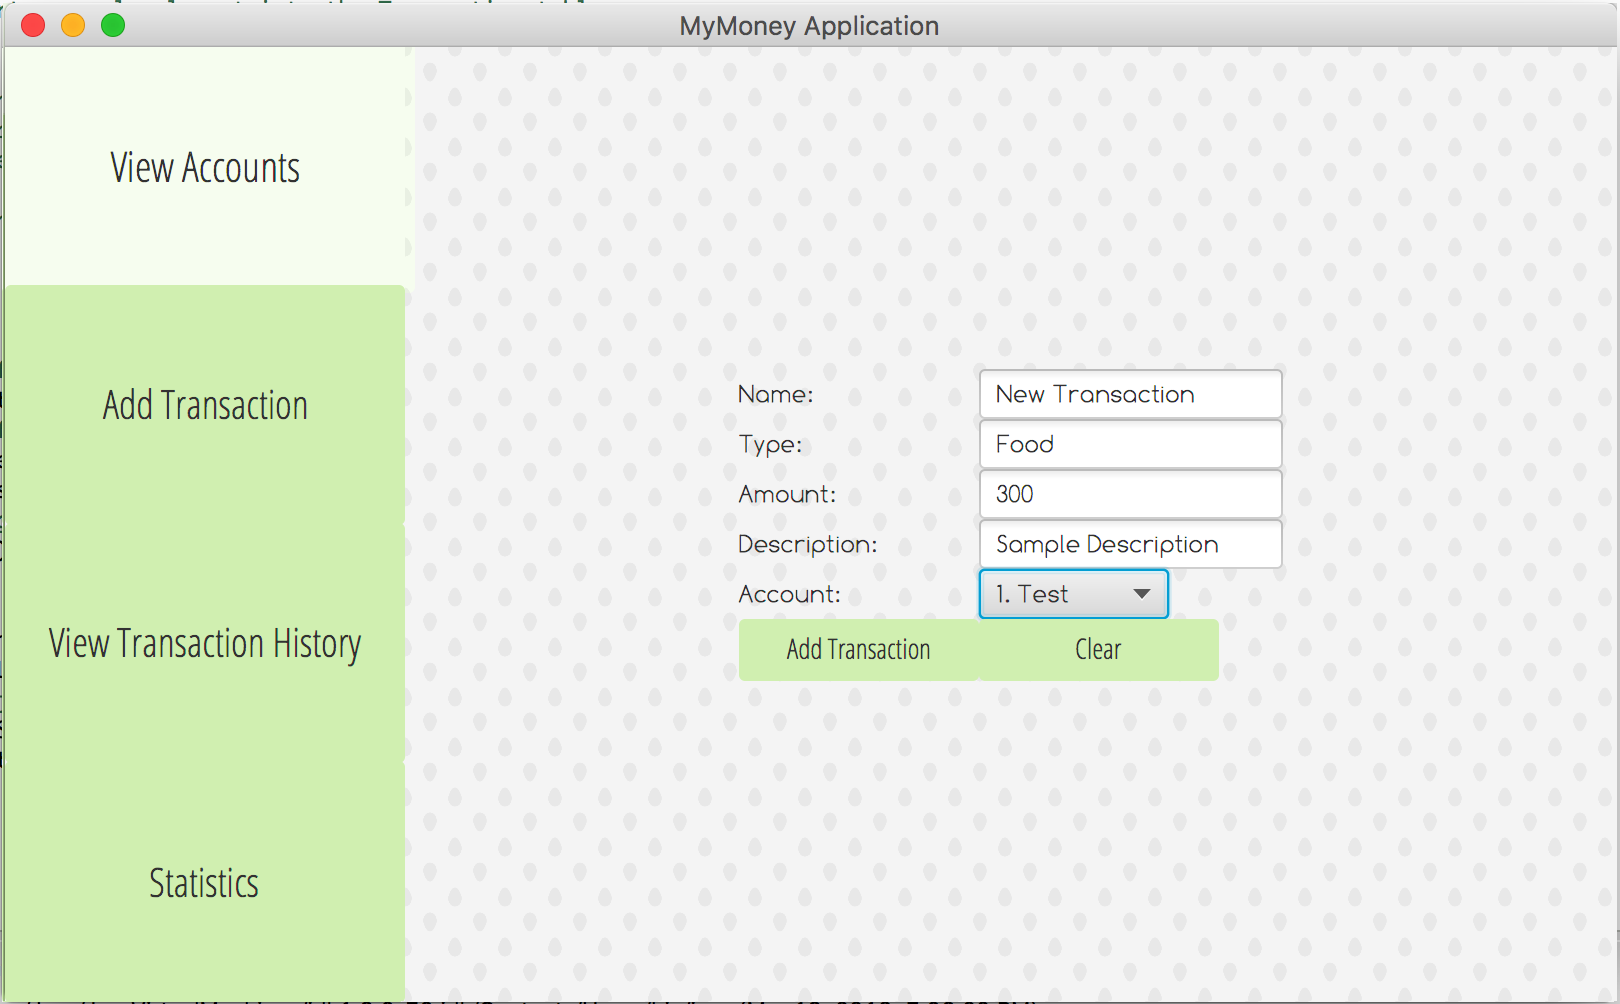
\includegraphics[scale=0.2]{transactionadd}

The Transaction Add view allows the user to add new Transactions to specified accounts.
From the Add view, the user can enter the name, type, amount, description, and associated account
of a transaction and insert it into the database.\\

From the Add view, the user is presented with two actions: Add and Clear.
When Clear is pressed, the TransactionAddController's ``clearTransaction''
method is called which removes any data filled into the view by the user.
The add action calls the ``addTransaction'' method of the TransactionAddController
to insert a new Transaction entry into the database using the TransactionDAO.

\section{Detailed Design} \label{sec:detail}

\iffalse 
https://tex.stackexchange.com/questions/94799/how-do-i-color-table-columns
\fi

\setcounter{secnumdepth}{4}

\titleformat{\paragraph}
{\normalfont\normalsize\bfseries}{\theparagraph}{0.9em}{}
\titlespacing*{\paragraph}
{0pt}{3.25ex plus 1ex minus .2ex}{1.5ex plus .2ex}

\newcommand{\graphicwidth}{18.5cm}
\newcommand{\colWidth}{12cm}
\definecolor{Gray}{gray}{0.85}
\definecolor{LightCyan}{rgb}{0.88,1,1}

Complete description of the system design, describing one subsystem separately in respective subsection.
UML class diagrams are to be used, as well as a short textual description describing the purpose of each class.

\subsection{Module $\langle Model\rangle$:}

\subsubsection{Detailed Design Diagram}


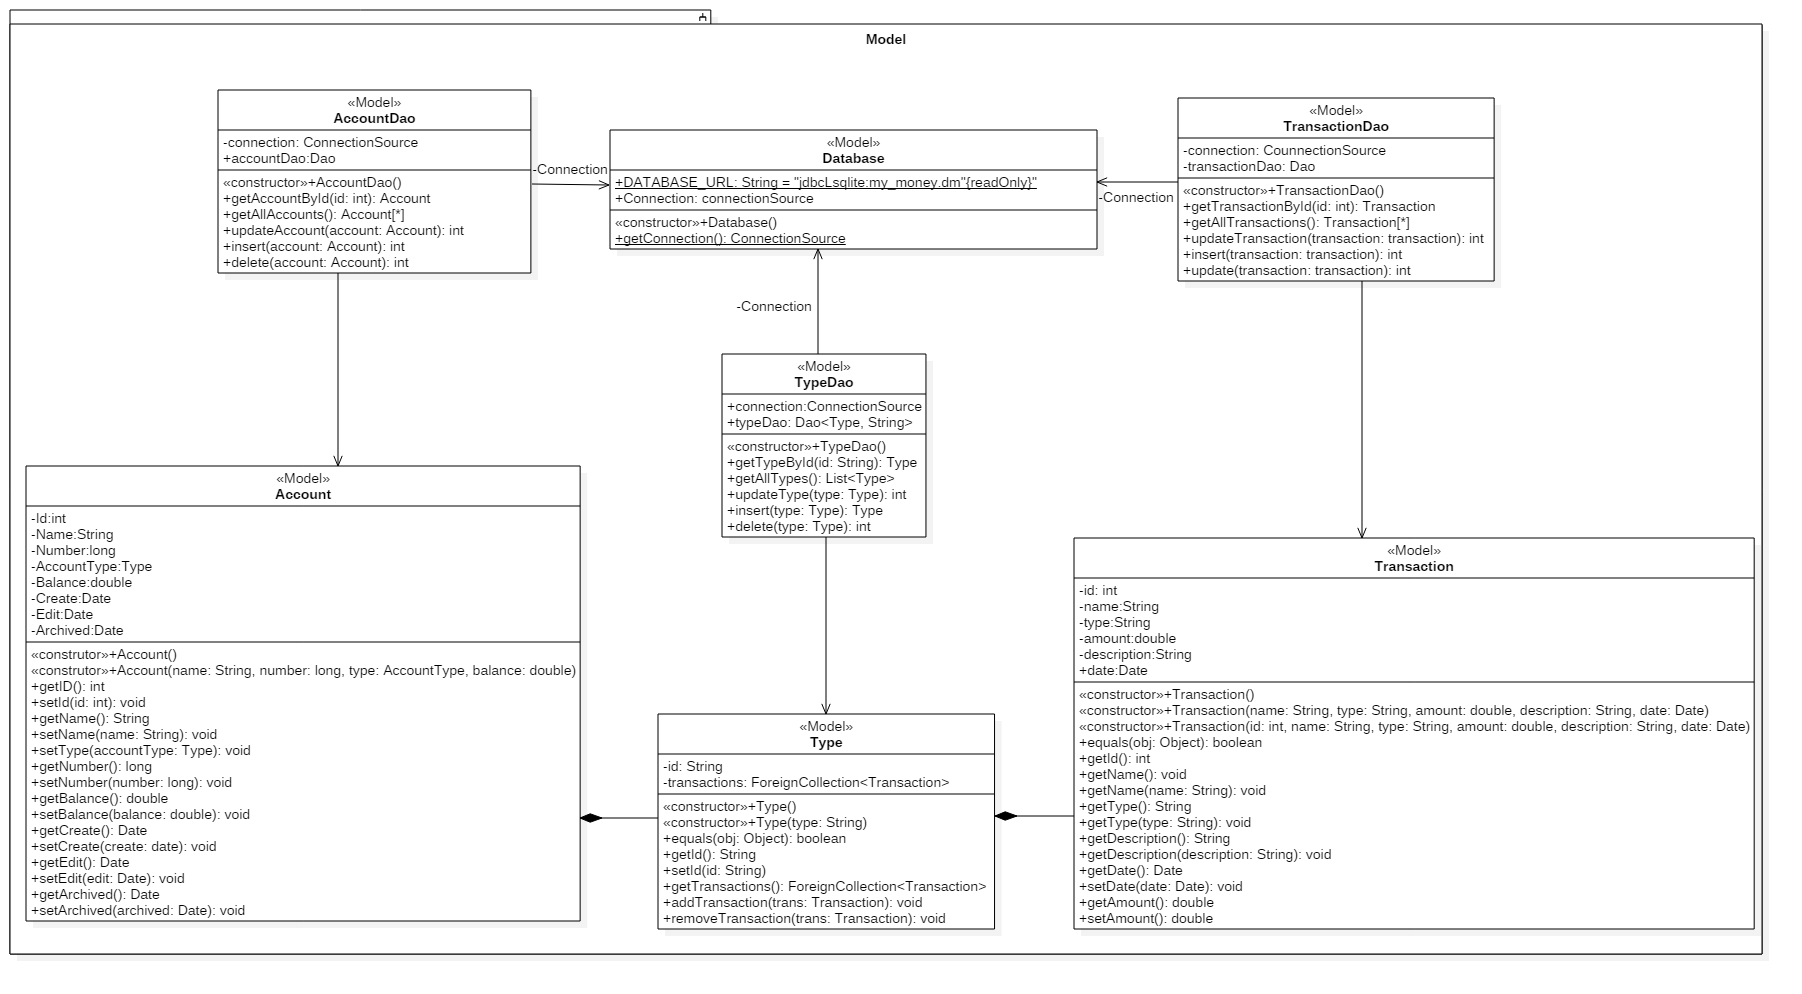
\includegraphics[width=\graphicwidth]{images/Model.png}
\captionof{figure}{Model Module Class Diagram}
The module of the model classes serves primarily to populate and create container objects. 'Account', 'Type' and 'Transaction' all have a 'Data Access Object' which draws information from the central database service using SQL queries. All information is used to generate views through access to Dao's by controllers.
\subsubsection{Units Description}






\paragraph{Class Transaction:} 
\begin{table}[H]
	\begin{tabular}{|a|p{15cm}|}
		\hline
		\rowcolor{LightCyan}
		{Class Name} & {Transaction} \\
		\hline
		Description & The Transaction class holds information on financial data that is to be sent to the server, processed by statistics, deleted or anything requiring data manipulation. \\
		\hline
		Attributes & 
		\begin{tabular}{| p{2cm} | p{2cm} | p{3cm} | p{6.45cm} |}
			\hline
			\rowcolor{lightgray}
			Visibility & Data Type & Name & Description \\
			\rowcolor{white}
			Private & int & id & An id of the transaction \\
			\hline
			Private & String & name & Name of user\\
			\hline
			Private & String & type & The type of action done \\
			\hline
			Private & double & amount & The quantity acted on \\
			\hline
			Private & String & description & A description of what it is \\
			\hline
			Private & Date & date & The date of the transaction \\
			\hline
		\end{tabular} \\
		\hline
		Methods & 		 
		\begin{tabular}{| p{2cm} | p{5cm} | p{6.9cm} |}
			\hline
			\rowcolor{gray}
			{Visibility} &{Name} & {Description} \\
			\hline
			\rowcolor{white}
			public &  Transaction() & default constructor\\
			\hline
			public &  Transaction(String name, String type, double amount, String description, Date date) & argument constructor\\
			\hline
			public & Transaction(int id, String name, String type, double amount, String description, Date date) & argument constructor with given id\\
			\hline
			public &  equals(Object obj) & Return a boolean from comparison\\
			\hline
			public &   getId() & return ID\\
			\hline
			public &  setId(int id) &  set the ID\\
			\hline
			public &  getName()  & get the name\\
			\hline
			public &  setName(String name)  & set the name\\
			\hline
			public &  getType() & get the type\\
			\hline
			public &  setType(String type) & set the type\\
			\hline
			public &  getDescription() & get the description\\
			\hline
			public & setDescription(String description) & set the description\\
			\hline
			public &  getDate() & get the date\\
			\hline
			public &  setDate(Date date)  & set the date\\
			\hline
			public &  getAmount() & get the amount\\
			\hline
			public &   setAmount(double amount) & set the amount\\
			\hline
			
		\end{tabular}								 
	\end{tabular}
\end{table}

\paragraph{Transaction Methods:}

\begin{tabular}{ |p{3cm}||p{\colWidth}|  }
	\hline
	Method Name & Transaction()\\
	\hline
	Class Name & Transaction\\
	\hline
	Functionality & default constructor\\
	\hline
	Input & -\\
	\hline
	Output & Transaction Class\\
	\hline
	Pseudo Code & -\\
	\hline
\end{tabular}



\begin{tabular}{ |p{3cm}||p{\colWidth}|  }
	\hline
	Method Name &  Transaction(String name, String type, double amount, String description, Date date)\\
	\hline
	Class Name & Transaction\\
	\hline
	Functionality & Argument Constructor\\
	\hline
	Input & Private field variables\\
	\hline
	Output & Transaction Class\\
	\hline
	Pseudo Code & *Set all class data fields to argument values\\
	\hline
\end{tabular}



\begin{tabular}{ |p{3cm}||p{\colWidth}|  }
	\hline
	Method Name & Transaction(int id, String name, String type, double amount, String description, Date date)\\
	\hline
	Class Name & Transaction\\
	\hline
	Functionality & Argument Constructor with id paramater\\
	\hline
	Input & Private field variables\\
	\hline
	Output & Transaction Class\\
	\hline
	Pseudo Code & BEGIN \\
	& *Set all class data fields to argument values\\
	& END \\
	\hline
\end{tabular}



\begin{tabular}{ |p{3cm}||p{\colWidth}|  }
	\hline
	Method Name &  equals(Object obj) \\
	\hline
	Class Name & Transaction\\
	\hline
	Functionality &  Return boolean based on variable comparision of Transaction objects\\
	\hline
	Input & - \\
	\hline
	Output & Boolean of transaction comparision\\
	\hline
	Pseudo Code & 	BEGIN \\
	& \\
	& Transaction t = (Transaction) obj \\
	& RETURN (t NOT null AND id EQUALS t.id AND name.equals(t.name) AND type.equals(t.type) \\
	& AND description.equals(t.description) AND amount EQUALS t.amount AND date.equals(t.date))\\
	& \\
	& END \\
	\hline
\end{tabular}



\begin{tabular}{ |p{3cm}||p{\colWidth}|  }
	\hline
	Method Name &  getId() \\
	\hline
	Class Name & Transaction\\
	\hline
	Functionality & return ID paramater\\
	\hline
	Input & -\\
	\hline
	Output & ID value\\
	\hline
	Pseudo Code& BEGIN \\
	& return this.id\\
	&END\\
	\hline
\end{tabular}



\begin{tabular}{ |p{3cm}||p{\colWidth}|  }
	\hline
	Method Name &  setId(int ID) \\
	\hline
	Class Name & Transaction\\
	\hline
	Functionality & sets the ID paramater\\
	\hline
	Input & ID integer\\
	\hline
	Output & -\\
	\hline
	Pseudo Code & BEGIN \\
	& this.id = ID\\
	&END\\
	\hline
\end{tabular}



\begin{tabular}{ |p{3cm}||p{\colWidth}|  }
	\hline
	Method Name &  getName() \\
	\hline
	Class Name & Transaction\\
	\hline
	Functionality & return account holder's name\\
	\hline
	Input & ID -\\
	\hline
	Output & Account holder's name\\
	\hline
	Pseudo Code& BEGIN \\ & return this.name\\
	&END\\
	\hline
\end{tabular}



\begin{tabular}{ |p{3cm}||p{\colWidth}|  }
	\hline
	Method Name &  setName(String name) \\
	\hline
	Class Name & Transaction\\
	\hline
	Functionality &  change the account holder's name\\
	\hline
	Input & ID Name string\\
	\hline
	Output & -\\
	\hline
	Pseudo Code& BEGIN \\ & this.name = name\\ & END\\
	\hline
\end{tabular}



\begin{tabular}{ |p{3cm}||p{\colWidth}|  }
	\hline
	Method Name &  getType() \\
	\hline
	Class Name & Transaction\\
	\hline
	Functionality &  Get the account type\\
	\hline
	Input & -\\
	\hline
	Output & Type string\\
	\hline
	Pseudo Code& BEGIN \\ & return this.type \\ & END\\
	\hline
\end{tabular}



\begin{tabular}{ |p{3cm}||p{\colWidth}|  }
	\hline
	Method Name &  setType(String type) \\
	\hline
	Class Name & Transaction\\
	\hline
	Functionality &  change the account type\\
	\hline
	Input & Type string\\
	\hline
	Output & -\\
	\hline
	Pseudo Code& BEGIN \\ & this.type = name\\ & END\\
	\hline
\end{tabular}



\begin{tabular}{ |p{3cm}||p{\colWidth}|  }
	\hline
	Method Name &  getDescription() \\
	\hline
	Class Name & Transaction\\
	\hline
	Functionality &  Return the description \\
	\hline
	Input & - \\
	\hline
	Output & Description string\\
	\hline
	Pseudo Code & BEGIN \\ & return this.description\\& END\\
	\hline
\end{tabular}



\begin{tabular}{ |p{3cm}||p{\colWidth}|  }
	\hline
	Method Name &  setDescription(String description) \\
	\hline
	Class Name & Transaction\\
	\hline
	Functionality &  Set the description \\
	\hline
	Input & Description string \\
	\hline
	Output & -\\
	\hline
	Pseudo Code& BEGIN \\ & this.description = description\\ & END\\
	\hline
\end{tabular}



\begin{tabular}{ |p{3cm}||p{\colWidth}|  }
	\hline
	Method Name &  getDate() \\
	\hline
	Class Name & Transaction\\
	\hline
	Functionality &  Get the date of the account\\
	\hline
	Input & -\\
	\hline
	Output & Date object of transaction\\
	\hline
	Pseudo Code& BEGIN \\ & return this.date\\ & END\\
	\hline
\end{tabular}



\begin{tabular}{ |p{3cm}||p{\colWidth}|  }
	\hline
	Method Name &  setDate(Date date) \\
	\hline
	Class Name & Transaction\\
	\hline
	Functionality &  Set the date of the account\\
	\hline
	Input & Date object of transaction\\
	\hline
	Output & -\\
	\hline& BEGIN \\
	Pseudo Code & this.date = date\\
	& END \\
	\hline
\end{tabular}



\begin{tabular}{ |p{3cm}||p{\colWidth}|  }
	\hline
	Method Name &  getAmount() \\
	\hline
	Class Name & Transaction\\
	\hline
	Functionality &  Get the amount returned.\\
	\hline
	Input & -\\
	\hline
	Output & return quantity transacted as a double\\
	\hline
	Pseudo Code& BEGIN \\ & return this.amount\\ & END \\
	\hline
\end{tabular}



\begin{tabular}{ |p{3cm}||p{\colWidth}|  }
	\hline
	Method Name &  setAmount(double amount) \\
	\hline
	Class Name & Transaction\\
	\hline
	Functionality &  Set the amount returned.\\
	\hline
	Input & amount transacted as a double\\
	\hline
	Output & -\\
	\hline
	Pseudo Code & BEGIN \\& this.amount = amount\\ & END\\
	\hline
\end{tabular}


\pagebreak

\paragraph{Class TransactionDao:}
\begin{table}[H]	
	\begin{tabular}{|a|p{15cm}|}
		\hline
		\rowcolor{LightCyan}
		{Class Name} & {TransactionDao} \\
		\hline
		Description & A transaction Dao is the way that transaction connect to the database. A Transaction Dao has reference to a set of Transaction objects and performs operations on networks with them.\\
		\hline
		Attributes & 
		\begin{tabular}{| p{1.8cm} | p{5.25cm} | p{3.4cm} | p{3.0cm} |}
			\hline
			\rowcolor{lightgray}
			Visibility & Data Type & Name & Description \\
			\rowcolor{white}
			private & ConnectionSource & connection & The address of a connection \\
			\hline
			private & Dao $\langle Transaction, Integer \rangle$ & transactionDao & the Transaction it is connected to \\
			\hline
		\end{tabular} \\
		\hline
		Methods & 		 
		\begin{tabular}{| p{2cm} | p{7cm} | p{4.9cm} |}
			\hline
			\rowcolor{gray}
			{Visibility} &{Name} & {Description} \\
			\hline
			\rowcolor{white}			
			public &  TransactionDao() & Default constructor\\
			\hline
			public &  getTransactionById(int id) & Return the record with a certain ID\\
			\hline
			public &  getAllTransactions(int number) & Return all Transaction objects contained\\
			\hline
			public &  updateTransaction(Transaction transaction) & updates an sql record\\
			\hline
			public &  insert(Transaction transaction) &  inserts a transaction\\
			\hline
			public &  delete(Transaction transaction) & Removes a transaction\\
			\hline
			
		\end{tabular}								 
	\end{tabular}
\end{table}
\paragraph{TransactionDao Methods:}
\begin{tabular}{ |p{3cm}||p{\colWidth}|  }
	\hline
	Method Name & TransactionDao()\\
	\hline
	Class Name & TransactionDao\\
	\hline
	Functionality & default constructor\\
	\hline
	Input & -\\
	\hline
	Output & TransactionDao Class\\
	\hline
	Pseudo Code & -\\
	\hline
\end{tabular}



\begin{tabular}{ |p{3cm}||p{\colWidth}|  }
	\hline
	Method Name & getTransactionById(int id)\\
	\hline
	Class Name & TransactionDao\\
	\hline
	Functionality & Get from the server a transaction of a certain ID\\
	\hline
	Input & Id to search for\\
	\hline
	Output & Transaction class found\\
	\hline
	Pseudo Code& BEGIN \\ & SQL Query the Database for this.id\\ &END\\
	\hline
\end{tabular}



\begin{tabular}{ |p{3cm}||p{\colWidth}|  }
	\hline
	Method Name & getAllTransactions()\\
	\hline
	Class Name & TransactionDao\\
	\hline
	Functionality & Returns a List of all Transactions in the database\\
	\hline
	Input & -\\
	\hline
	Output & Transaction List\\
	\hline
	Pseudo Code& BEGIN \\ & SQL Query the Database for any values\\ & END\\
	\hline
\end{tabular}\\



\begin{tabular}{ |p{3cm}||p{\colWidth}|  }
	\hline
	Method Name & updateTransaction(Transaction transaction)\\
	\hline
	Class Name & TransactionDao\\
	\hline
	Functionality & Find a transaction by ID and update the records\\
	\hline
	Input & Transaction to update\\
	\hline
	Output & integer success code\\
	\hline
	Pseudo Code& BEGIN\\ & SQL Query the Database to update certain ID values\\ & END \\
	\hline
\end{tabular}


\begin{tabular}{ |p{3cm}||p{\colWidth}|  }
	\hline
	Method Name & insert(Transaction transaction)\\
	\hline
	Class Name & TransactionDao\\
	\hline
	Functionality & Inserts a record into the database\\
	\hline
	Input & Transaction to insert\\
	\hline
	Output & Integer success code\\
	\hline
	Pseudo Code&BEGIN\\ & SQL Query the Database to insert certain Transactions\\ & END \\
	\hline
\end{tabular}



\begin{tabular}{ |p{3cm}||p{\colWidth}|  }
	\hline
	Method Name & delete(Transaction transaction)\\
	\hline
	Class Name & TransactionDao\\
	\hline
	Functionality & Delete a record from the database\\
	\hline
	Input & Transaction to delete\\
	\hline
	Output & Integer success code\\
	\hline
	Pseudo Code&BEGIN\\ & SQL Query the Database to delete certain Transactions\\&END\\
	\hline
\end{tabular}            

\pagebreak

\paragraph{Class Type}
\begin{table}[H]
	\begin{tabular}{|a|p{15cm}|}
		\hline
		\rowcolor{LightCyan}
		{Class Name} & {Type} \\
		\hline
		Description & The Type class represents the different sorts of account types users can create. Types are associated with transactions in that they hold a ForeignCollection of Transactions associated with the Type\\
		\hline
		Attributes & 
		\begin{tabular}{| p{1.8cm} | p{2.25cm} | p{6.4cm} | p{3.0cm} |}
			\rowcolor{lightgray}
			Visibility & Data Type & Name & Description \\
			\hline
			\rowcolor{white}
			private & String & id & The unique identifier of a Type \\
			\hline
			private & ForeignCollection$\langle Transaction \rangle$ & transactions & A set of transactions associated with the class. \\
			\hline		
		\end{tabular} \\
		\hline
		Methods & 		 
		\begin{tabular}{| p{2cm} | p{5cm} | p{6.9cm} |}
			\hline
			\rowcolor{gray}
			{Visibility} &{Name} & {Description} \\
			\hline
			\rowcolor{white}			
			public & Type() & Default constructor\\
			\hline
			public &  Type(String type) & Constructor specifying Type\\
			\hline
			public &  equals(Object obj) & Checks the equivalence against this Object and argument Object\\
			\hline
			public &  getId() & Returns Id string\\
			\hline
			public &  setId(String id) &  Sets the Id string\\
			\hline
			public &  getTransactions() & Returns the set of transactions associated with class\\
			\hline
			public &  addTransaction(Transaction trans) & Adds another transaction to the class\\
			\hline
			public &  removeTransaction(Transaction trans) & Removes a transaction associated with the class\\
			\hline		
		\end{tabular}								 
	\end{tabular}
\end{table}

\paragraph{Type Methods:}
\begin{tabular}{ |p{3cm}||p{\colWidth}|  }
	\hline
	Method Name & Type()\\
	\hline
	Class Name & Type\\
	\hline
	Functionality & Default constructor to create a Type object\\
	\hline
	Input & -\\
	\hline
	Output & Type Object\\
	\hline
	Pseudo Code&BEGIN\\&END\\
	\hline
\end{tabular}            

\begin{tabular}{ |p{3cm}||p{\colWidth}|  }
	
	\hline
	Method Name & Type(String type)\\
	\hline
	Class Name & Type\\
	\hline
	Functionality & Argument constructor to create a Type object\\
	\hline
	Input & Type string\\
	\hline
	Output & Type Object\\
	\hline
	Pseudo Code&BEGIN\\ & this.type = type\\&END\\
	\hline
\end{tabular}        

\begin{tabular}{ |p{3cm}||p{\colWidth}|  }
	\hline
	Method Name & equals(Object obj)\\
	\hline
	Class Name & Type\\
	\hline
	Functionality & Check equivalence between objects\\
	\hline
	Input & Object to compare\\
	\hline
	Output & Boolean of comparison\\
	\hline
	Pseudo Code & BEGIN\\
	& Type t = (Type) obj \\
	& RETURN t NOT null AND id.equals(t.id) \\
	& END\\
	\hline
\end{tabular}        

\begin{tabular}{ |p{3cm}||p{\colWidth}|  }
	\hline
	Method Name & getID()\\
	\hline
	Class Name & Type\\
	\hline
	Functionality & Return ID of Type\\
	\hline
	Input & -\\
	\hline
	Output & Type ID\\
	\hline
	Pseudo Code&BEGIN\\ & return this.id\\&END\\
	\hline
\end{tabular}        

\begin{tabular}{ |p{3cm}||p{\colWidth}|  }
	\hline
	Method Name & setId()\\
	\hline
	Class Name & Type\\
	\hline
	Functionality & Set ID value of type\\
	\hline
	Input & Type ID\\
	\hline
	Output & -\\
	\hline
	Pseudo Code&BEGIN\\ & this.id = id\\&END\\
	\hline
\end{tabular}      

\begin{tabular}{ |p{3cm}||p{\colWidth}|  }
	\hline
	Method Name & getTransactions()\\
	\hline
	Class Name & Type\\
	\hline
	Functionality & Returns transactions associated with the type\\
	\hline
	Input & -  \\
	\hline
	Output & Foreign Collection of Transactions\\
	\hline
	Pseudo Code&BEGIN\\ & return this.transactions\\&END\\
	\hline
\end{tabular}        

\begin{tabular}{ |p{3cm}||p{\colWidth}|  }
	\hline
	Method Name & addTransaction(Transaction trans)\\
	\hline
	Class Name & Type\\
	\hline
	Functionality & Adds a transaction value to the transaction array\\
	\hline
	Input & Transaction to add\\
	\hline
	Output & - \\
	\hline
	Pseudo Code&BEGIN\\ & transactions.add(trans)\\&END\\
	\hline
\end{tabular}        

\begin{tabular}{ |p{3cm}||p{\colWidth}|  }
	\hline
	Method Name & removeTransaction(Transaction trans)\\
	\hline
	Class Name & Type\\
	\hline
	Functionality & Remove a transaction value from the transaction array\\
	\hline
	Input & Transaction to remove\\
	\hline
	Output & - \\
	\hline
	Pseudo Code&BEGIN\\ & transactions.remove(trans)\\&END\\
	\hline
\end{tabular}        

\paragraph{Class TypeDao}
\begin{table}[H]
	\begin{tabular}{|a|p{15cm}|}
		\hline
		\rowcolor{LightCyan}
		{Class Name} & {TypeDao} \\
		\hline
		Description & The TypeDao is the class which communicates Type information back and forth with the database.\\
		\hline
		Attributes & 
		\begin{tabular}{| p{1.8cm} | p{3.25cm} | p{5.4cm} | p{3.0cm} |}
			\hline
			\rowcolor{lightgray}
			Visibility & Data Type & Name & Description \\
			\hline
			\rowcolor{white}
			public & connection & ConnectionSource & A connection point with the database \\
			\hline
			public & Dao$\langle Type, String \rangle$  & typeDao  & A set of Type's being connected to the database \\	
			\hline	
		\end{tabular} \\
		\hline
		Methods & 		 
		\begin{tabular}{| p{2cm} | p{5cm} | p{6.9cm} |}
			\hline
			\rowcolor{gray}
			{Visibility} &{Name} & {Description} \\
			\hline
			\rowcolor{white}			
			public &  TypeDao() & Default constructor\\
			\hline
			public &  getTypeById(String id)&Gets Types with certain Ids\\
			\hline
			public &  getAllTypes() & Gets all data\\
			\hline
			public &  updateType(Type type) & update the Type with the server\\
			\hline
			public &  insert(Type type) & insert a Type with the server\\
			\hline
			public &  delete(Type type) & delete the Type with the server\\ 
			\hline
			
		\end{tabular}								 
	\end{tabular}
\end{table}
\paragraph{TypeDao Methods:}

\begin{tabular}{ |p{3cm}||p{\colWidth}|  }
	\hline
	Method Name & TypeDao()\\
	\hline
	Class Name & TypeDao\\
	\hline
	Functionality & Default constructor to create a TypeDao object\\
	\hline
	Input & -\\
	\hline
	Output & TypeDao Object\\
	\hline
	Pseudo Code & -\\
	\hline
\end{tabular}            

\begin{tabular}{ |p{3cm}||p{\colWidth}|  }
	\hline
	Method Name &  getTypeById(String id)\\
	\hline
	Class Name & Type\\
	\hline
	Functionality & Returns all types of certain Id\\
	\hline
	Input & Id to find\\
	\hline
	Output & Type Object\\
	\hline
	Pseudo Code &BEGIN\\& SQL Query database for Id string\\&END\\
	\hline
\end{tabular}            

\begin{tabular}{ |p{3cm}||p{\colWidth}|  }
	\hline
	Method Name &  getAllTypes()\\
	\hline
	Class Name & Type\\
	\hline
	Functionality & Returns all Types in database\\
	\hline
	Input & -\\
	\hline
	Output & List of Type Object \\
	\hline
	Pseudo Code&BEGIN\\ & SQL Query database for all Types\\&END\\
	\hline
\end{tabular}    

\begin{tabular}{ |p{3cm}||p{\colWidth}|  }
	\hline
	Method Name &  updateType(Type type)\\
	\hline
	Class Name & Type\\
	\hline
	Functionality & Updates types of certain Id\\
	\hline
	Input & Type to find\\
	\hline
	Output & Integer success code\\
	\hline
	Pseudo Code&BEGIN\\ & SQL Query database to update Type\\&END\\
	\hline
\end{tabular}    

\begin{tabular}{ |p{3cm}||p{\colWidth}|  }
	\hline
	Method Name &  insert(Type type)\\
	\hline
	Class Name & Type\\
	\hline
	Functionality & Inserts Types into database\\
	\hline
	Input & Type to insert\\
	\hline
	Output & integer success code\\
	\hline
	Pseudo Code&BEGIN\\ & SQL Query to insert data into database\\&END\\
	\hline
\end{tabular}    

\begin{tabular}{ |p{3cm}||p{\colWidth}|  }
	\hline
	Method Name &  delete(Type type)\\
	\hline
	Class Name & Type\\
	\hline
	Functionality & Delete Types from database\\
	\hline
	Input & Type to remove\\
	\hline
	Output & integer success code\\
	\hline
	Pseudo Code&BEGIN\\ & SQL Query to remove data from database\\&END\\
	\hline
\end{tabular}  



\paragraph{Class Account}
\begin{table}[H]
	\begin{tabular}{|a|p{15cm}|}
		\hline
		\rowcolor{LightCyan}
		{Class Name} & {Account} \\
		\hline
		Description & An account holds a user's specific information on who they are and what their overall finances are like. 
		It is connected to the database by AccountDao\\
		\hline
		
		Attributes & 
		\begin{tabular}{| p{2cm} | p{2cm} | p{3cm} | p{6.45cm} |}
			\hline
			\rowcolor{lightgray}
			Visibility & Data Type & Name & Description \\
			\hline
			\rowcolor{white}
			private & int & id  & The unique identifier of Account \\
			\hline
			private & String & Name  & Name of the account holder \\
			\hline
			private & long & Number  & Account number \\
			\hline
			private & Type & AccountType  & Type of account \\
			\hline
			private & double & Balance  & Holdings of account \\
			\hline
			private & Date & Create  & Date created of account \\
			\hline
			private & Date & Edit  & Date edited of account \\
			\hline
			private & Date & Archived  & Date archived of account  \\
			\hline
		\end{tabular} \\
		\hline
		Methods & 		 
		\begin{tabular}{| p{2cm} | p{5cm} | p{6.9cm} |}
			\hline
			\rowcolor{gray}
			{Visibility} &{Name} & {Description} \\
			\hline
			\rowcolor{white}			
			public & Account() & Default Account constructor\\
			\hline
			public &  Account(name:String, number:long, type:AccountType, balance:double) & Argument Account constructor\\
			\hline
			public &  getId() & Returns unique identifier\\
			\hline
			public &  setId(int id) & Sets unique identifier\\
			\hline
			public &  getName() & Returns name of account holder\\
			\hline
			public &  setName(name:String) & sets name of account holder\\
			\hline
			public &  getType() & sets the account Type\\
			\hline
			public &  setType(accountType:Type) & sets the account Type\\
			\hline
			public &  getNumber() & Returns account number\\
			\hline
			public &  setNumber(number: long) & Sets account number\\
			\hline
			public &  getBalance() & Returns account holdings\\
			\hline
			public &  setBalance(balance:double) & Sets the account balances\\
			\hline
			public &  getCreate() & Get the creation date\\
			\hline
			public &  setCreate(create:Date) & Set the creation date\\
			\hline
			public &  getEdit() & Gets edited date\\
			\hline
			public &  setEdit(edited:Date) & Sets edited date\\
			\hline
			public &  getArchived() & Returns date archived\\
			\hline
			public &  setArchived(archived:Date) & Sets date archived\\
			\hline
			
		\end{tabular}								 
	\end{tabular}
\end{table}
\paragraph{Account Methods:}

\begin{tabular}{ |p{3cm}||p{\colWidth}|  }
	\hline
	Method Name &  Account()\\
	\hline
	Class Name & Account\\
	\hline
	Functionality & Default Account constructor\\
	\hline
	Input & -\\
	\hline
	Output & Account Object\\
	\hline
	Pseudo Code & -\\
	\hline
\end{tabular}  

\begin{tabular}{ |p{3cm}||p{\colWidth}|  }
	\hline
	Method Name &  Account(name:String, number:long, type:AccountType, balance:double)\\
	\hline
	Class Name & Account\\
	\hline
	Functionality & Argument Account constructor\\
	\hline
	Input & Private fields to be set\\
	\hline
	Output & Account Object\\
	\hline
	Pseudo Code&BEGIN\\ & Set each private field with the respective arguments\\&END\\
	\hline
\end{tabular}  

\begin{tabular}{ |p{3cm}||p{\colWidth}|  }
	\hline
	Method Name &  getId()\\
	\hline
	Class Name & Account\\
	\hline
	Functionality & Gets account ID\\
	\hline
	Input & -\\
	\hline
	Output & Account Id\\
	\hline
	Pseudo Code&BEGIN\\ & return this.id\\&END\\
	\hline
\end{tabular}  

\begin{tabular}{ |p{3cm}||p{\colWidth}|  }
	\hline
	Method Name &  setId(int id)\\
	\hline
	Class Name & Account\\
	\hline
	Functionality & Sets account ID\\
	\hline
	Input & Account Id \\
	\hline
	Output & -\\
	\hline
	Pseudo Code&BEGIN\\ & this.id = id\\&END\\
	\hline
\end{tabular} 

\begin{tabular}{ |p{3cm}||p{\colWidth}|  }
	\hline
	Method Name &  getName()\\
	\hline
	Class Name & Account\\
	\hline
	Functionality & Gets account Name\\
	\hline
	Input & -\\
	\hline
	Output & Account Name\\
	\hline
	Pseudo Code&BEGIN\\ & return this.name\\&END\\
	\hline
\end{tabular}  

\begin{tabular}{ |p{3cm}||p{\colWidth}|  }
	\hline
	Method Name &  setName(String name)\\
	\hline
	Class Name & Account\\
	\hline
	Functionality & Sets account Name\\
	\hline
	Input & Account Name\\
	\hline
	Output & -\\
	\hline
	Pseudo Code&BEGIN\\ & this.name = name\\&END\\
	\hline
\end{tabular}  

\begin{tabular}{ |p{3cm}||p{\colWidth}|  }
	\hline
	Method Name &  getType()\\
	\hline
	Class Name & Account\\
	\hline
	Functionality & Gets account Type\\
	\hline
	Input & -\\
	\hline
	Output & Account Type\\
	\hline
	Pseudo Code &BEGIN\\& return this.type\\&END\\
	\hline
\end{tabular}  

\begin{tabular}{ |p{3cm}||p{\colWidth}|  }
	\hline
	Method Name &  setType(Type type)\\
	\hline
	Class Name & Account\\
	\hline
	Functionality & Sets account Type\\
	\hline
	Input & Account Type\\
	\hline
	Output & -\\
	\hline
	Pseudo Code&BEGIN\\ & this.type = type\\&END\\
	\hline
\end{tabular}  

\begin{tabular}{ |p{3cm}||p{\colWidth}|  }
	\hline
	Method Name &  getNumber()\\
	\hline
	Class Name & Account\\
	\hline
	Functionality & Gets account number\\
	\hline
	Input & -\\
	\hline
	Output & Account Number\\
	\hline
	Pseudo Code &BEGIN\\& return this.number\\&END\\
	\hline
\end{tabular}  

\begin{tabular}{ |p{3cm}||p{\colWidth}|  }
	\hline
	Method Name &  getNumber(long number)\\
	\hline
	Class Name & Account\\
	\hline
	Functionality & Sets account number\\
	\hline
	Input & Account Number\\
	\hline
	Output & -\\
	\hline
	Pseudo Code&BEGIN\\ & this.number = number\\&END\\
	\hline
\end{tabular}  

\begin{tabular}{ |p{3cm}||p{\colWidth}|  }
	\hline
	Method Name &  setNumber()\\
	\hline
	Class Name & Account\\
	\hline
	Functionality & Sets account number\\
	\hline
	Input & Account Number\\
	\hline
	Output & -\\
	\hline
	Pseudo Code&BEGIN\\ & this.number = number\\&END\\
	\hline
\end{tabular}   

\begin{tabular}{ |p{3cm}||p{\colWidth}|  }
	\hline
	Method Name &  getBalance()\\
	\hline
	Class Name & Account\\
	\hline
	Functionality & Gets account balance\\
	\hline
	Input & -\\
	\hline
	Output & Account Balance\\
	\hline
	Pseudo Code &BEGIN\\& return this.balance\\&END\\
	\hline
\end{tabular}

\begin{tabular}{ |p{3cm}||p{\colWidth}|  }
	\hline
	Method Name &  setBalance()\\
	\hline
	Class Name & Account\\
	\hline
	Functionality & Sets account balance\\
	\hline
	Input & Account Balance\\
	\hline
	Output & -\\
	\hline
	Pseudo Code &BEGIN\\& this.balance = balance\\&END\\
	\hline
\end{tabular}

\begin{tabular}{ |p{3cm}||p{\colWidth}|  }
	\hline
	Method Name &  getCreate()\\
	\hline
	Class Name & Account\\
	\hline
	Functionality & Gets account creation Date\\
	\hline
	Input & -\\
	\hline
	Output & Account creation Date\\
	\hline
	Pseudo Code&BEGIN\\ & return this.create\\&END\\
	\hline
\end{tabular}

\begin{tabular}{ |p{3cm}||p{\colWidth}|  }
	\hline
	Method Name &  setCreate(create)\\
	\hline
	Class Name & Account\\
	\hline
	Functionality & Sets account creation Date\\
	\hline
	Input & Account creation Date\\
	\hline
	Output & -\\
	\hline
	Pseudo Code&BEGIN\\ & this.create = create\\&END\\
	\hline
\end{tabular}

\begin{tabular}{ |p{3cm}||p{\colWidth}|  }
	\hline
	Method Name &  getEdit()\\
	\hline
	Class Name & Account\\
	\hline
	Functionality & Gets account edit Date\\
	\hline
	Input & -\\
	\hline
	Output & Account edit Date\\
	\hline
	Pseudo Cod&BEGIN\\e & return this.edited\\&END\\
	\hline
\end{tabular}

\begin{tabular}{ |p{3cm}||p{\colWidth}|  }
	\hline
	Method Name &  setEdit(edited)\\
	\hline
	Class Name & Account\\
	\hline
	Functionality & Sets account edit Date\\
	\hline
	Input & Account edit Date\\
	\hline
	Output & -\\
	\hline
	Pseudo Code&BEGIN\\ & this.edited = edited\\&END\\
	\hline
\end{tabular}

\begin{tabular}{ |p{3cm}||p{\colWidth}|  }
	\hline
	Method Name &  getArchived()\\
	\hline
	Class Name & Account\\
	\hline
	Functionality & Gets account archived Date\\
	\hline
	Input & -\\
	\hline
	Output & Account archive Date\\
	\hline
	Pseudo Code&BEGIN\\ & return this.archived\\&END\\
	\hline
\end{tabular}

\begin{tabular}{ |p{3cm}||p{\colWidth}|  }
	\hline
	Method Name &  setArchived(archived)\\
	\hline
	Class Name & Account\\
	\hline
	Functionality & Sets account archived Date\\
	\hline
	Input & Account archive Date\\
	\hline
	Output & -\\
	\hline
	Pseudo Code&BEGIN\\ & this.archived = archived\\&END\\
	\hline
\end{tabular}

\pagebreak


\paragraph{Class AccountDao}
\begin{table}
	\begin{tabular}{|a|p{15cm}|}
		\hline
		\rowcolor{LightCyan}
		{Class Name} & {AccountDao} \\
		\hline
		Description & An Account Dao is the way that account info is transmitted to and from the database. \\
		\hline
		Attributes & 
		\begin{tabular}{| p{2cm} | p{4.0cm} | p{3.0cm} | p{4.45cm} |}
			\hline
			\rowcolor{lightgray}
			Visibility & Data Type & Name & Description \\
			\hline
			\rowcolor{white}
			private & ConnectionSource & connection & The address of a connection \\
			\hline
			private & Dao & AccountDao & The Dao connecting to the database \\
			\hline
		\end{tabular} \\
		\hline
		Methods & 		 
		\begin{tabular}{| p{2cm} | p{6cm} | p{5.9cm} |}
			\hline
			\rowcolor{gray}
			{Visibility} &{Name} & {Description} \\
			\hline
			\rowcolor{white}			
			public & AccountDao() & Default constructor\\
			\hline
			public &  getAccountById(id:int) & Return the account with a certain ID\\
			\hline
			public &  getAllAccounts() & Return an array of all accounts\\
			\hline
			public &  updateAccount(account:Account)& Updates an sql record\\
			\hline
			public &  insert(account:Account) &  Inserts an account\\
			\hline
			public &  delete(account:Account) & Removes an account\\
			\hline		
		\end{tabular}								 
	\end{tabular}
\end{table}

\paragraph{AccountDao Methods:}

\begin{tabular}{ |p{3cm}||p{\colWidth}|  }
	\hline
	Method Name &  AccountDao()\\
	\hline
	Class Name & AccountDao\\
	\hline
	Functionality & Default AccountDao constructor. Connects to database and sets connection paramaters.\\
	\hline
	Input & -\\
	\hline
	Output & AccountDao object\\
	\hline
	Pseudo Code & -\\
	\hline
\end{tabular}    


\begin{tabular}{ |p{3cm}||p{\colWidth}|  }
	\hline
	Method Name &  getAccountById(id:int)\\
	\hline
	Class Name & AccountDao\\
	\hline
	Functionality & Get and account of certain ID from database\\
	\hline
	Input & Id to search\\
	\hline
	Output &  Account found\\
	\hline
	Pseudo Code&BEGIN\\ & SQL Query to find date from database\\&END\\
	\hline
\end{tabular}    

\begin{tabular}{ |p{3cm}||p{\colWidth}|  }
	\hline
	Method Name &  getAllAccounts()\\
	\hline
	Class Name & AccountDao\\
	\hline
	Functionality & Get all accounts from database\\
	\hline
	Input & Accounts to search\\
	\hline
	Output & List of accounts found\\
	\hline
	Pseudo Code &BEGIN\\& SQL Query to find account from database\\&END\\
	\hline
\end{tabular}    

\begin{tabular}{ |p{3cm}||p{\colWidth}|  }
	\hline
	Method Name &  updateAccount(Account account)\\
	\hline
	Class Name & AccountDao\\
	\hline
	Functionality & Update account in database\\
	\hline
	Input & Account to update\\
	\hline
	Output & Integer success code\\
	\hline
	Pseudo Code&BEGIN\\ & SQL Query to find account from database\\&END\\
	\hline
\end{tabular}


\begin{tabular}{ |p{3cm}||p{\colWidth}|  }
	\hline
	Method Name &  insert(Account account)\\
	\hline
	Class Name & AccountDao\\
	\hline
	Functionality & Insert account in database\\
	\hline
	Input & Account to update\\
	\hline
	Output & Integer success code\\
	\hline
	Pseudo Code & SQL Query to insert account into database\\&END\\
	\hline
\end{tabular}

\begin{tabular}{ |p{3cm}||p{\colWidth}|  }
	\hline
	Method Name &  delete(Account account)\\
	\hline
	Class Name & AccountDao\\
	\hline
	Functionality & Delete account from database\\
	\hline
	Input & Account to Delete\\
	\hline
	Output & Integer success code\\
	\hline
	Pseudo Code &BEGIN\\& SQL Query to Delete account from database\\&END\\
	\hline
\end{tabular}

\paragraph{Class Database}
\begin{table}[H]
	\begin{tabular}{|a|p{15cm}|}
		\hline
		\rowcolor{LightCyan}
		{Class Name} & {Database} \\
		\hline
		Description & The database contains all information for users from accounts and types to transactions.\\
		\hline
		Attributes & 
		\begin{tabular}{| p{2cm} | p{3.5cm} | p{4.5cm} | p{3.45cm} |}
			\hline
			\rowcolor{lightgray}
			Visibility & Data Type & Name & Description \\
			\hline
			\rowcolor{white}
			static public & String & DATABASE\_URL & the URL of the database\\
			\hline
			public & ConnectionSource & connection & The address of a connection \\
			\hline		
		\end{tabular} \\
		\hline
		Methods & 		 
		\begin{tabular}{| p{2cm} | p{5cm} | p{6.9cm} |}
			\hline
			\rowcolor{gray}
			{Visibility} &{Name} & {Description} \\
			\hline
			\rowcolor{white}			
			public & Database() & Default constructor\\
			\hline
			public &  getConnection() & return connection to the database\\
			\hline	
		\end{tabular}								 
	\end{tabular}
\end{table}

\paragraph {Database Methods:}

\begin{tabular}{ |p{3cm}||p{\colWidth}|  }
	\hline
	Method Name &  Database()\\
	\hline
	Class Name & Database\\
	\hline
	Functionality & Default Database constructor.\\
	\hline
	Input & -\\
	\hline
	Output & Database object\\
	\hline
	Pseudo Code & -\\
	\hline
\end{tabular}    

\begin{tabular}{ |p{3cm}||p{\colWidth}|  }
	\hline
	Method Name &  getConnection()\\
	\hline
	Class Name & Database\\
	\hline
	Functionality & returns a connection to the database.\\
	\hline
	Input & -\\
	\hline
	Output & Database connection\\
	\hline
	Pseudo Code & return connection\\
	\hline
\end{tabular}  

\subsection{Module $\langle View\rangle$:}
\subsubsection{Detailed Design Diagram}

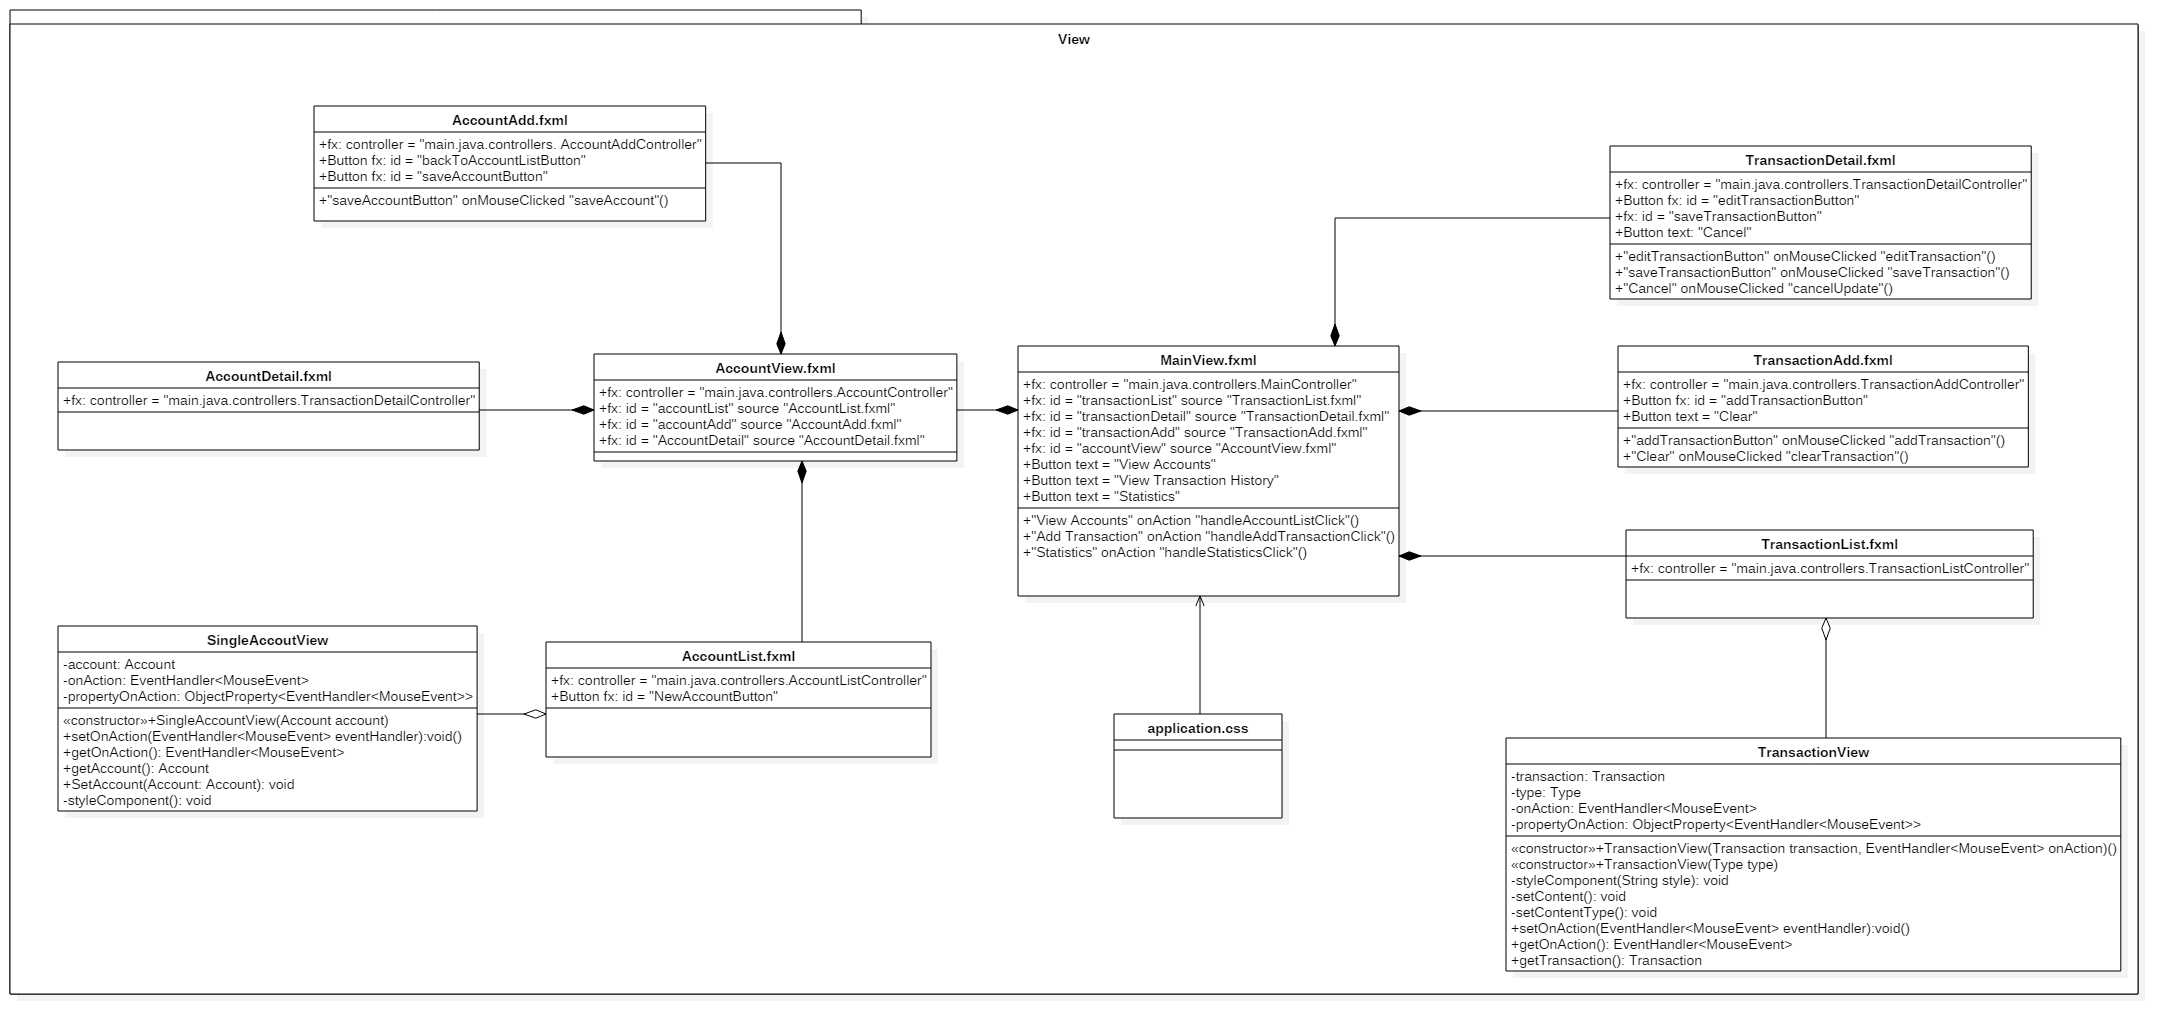
\includegraphics[width=\graphicwidth]{images/View.png}
\captionof{figure}{View Module Class Diagram}
The module of the view classes serves as a way to allow the user to visualize his/her data and allow him/her to manipulate it in the ways the application allows. By clicking on screen objects the user can transfer to different views. Views are .fxml files generated by a FXMLLoader class.
\subsubsection{Units Description}
\paragraph{XML MainView.fxml}
\begin{table}[H]
	\begin{tabular}{|a|p{15cm}|}
		\hline
		\rowcolor{LightCyan}
		{Class Name} & {MainView.fxml} \\
		\hline
		Description & MainView.fxml is the XML file that generates the main navigation screen. It contains within it as sources the other views and shifts to them when certain controller functions are called\\
		\hline
		Attributes & 
		\begin{tabular}{| p{1.5cm} | p{2.0cm} | p{6.5cm} | p{3.45cm} |}
			\hline
			\rowcolor{lightgray}
			Visibility & Data Type & Name & Description \\
			\hline	
			\rowcolor{white}	
			\hline	
			public & fx:controller  & main.java.controllers.MainController & Reference to controller\\
			\hline		
			public & fx:id  &  "transactionList"source"TransactionList.fxml" & Id of item containing the Transactionlist.fxml\\
			\hline		
			public & fx:id  & "transactionDetail"source"TransactionDetail.fxml" & Id of item containing the TransactionDetail.fxml\\	
			\hline		
			public & fx:id  & "transactionAdd" source "TransactionAdd.fxml" & Id of item containing the TransactionAdd.fxml\\	
			\hline		
			public & fx:id  & "accountView" source "AccountView.fxml" & Id of item containing the AccountView.fxml\\	
			\hline		
			public & Button  &  "View Accounts" & A button that can be pressed shifting to account view\\	
			\hline		
			public & Button  &  "View Transaction History" & button that can be pressed shifting to a transaction view\\	
			\hline		
			public & Button  & "Statistics" & button that can be pressed shifting to a statistical view\\	
			\hline		
		\end{tabular} \\
		\hline
	\end{tabular}
\end{table}

\paragraph{XML TransactionList.fxml}
\begin{table}[H]
	\begin{tabular}{|a|p{15cm}|}
		\hline
		\rowcolor{LightCyan}
		{Class Name} & {TransactionList.fxml} \\
		\hline
		Description & A view containing items the user can interact with to manipulate transaction settings\\
		\hline
		Attributes & 
		\begin{tabular}{| p{1.5cm} | p{2.0cm} | p{6.5cm} | p{3.45cm} |}
			\hline
			\rowcolor{lightgray}
			Visibility & Data Type & Name & Description \\
			\hline
			\rowcolor{white}
			public & fx: controller & "main.java.controllers.TransactionAddController" & Reference to controller\\
			\hline
		\end{tabular} \\
		\hline								 
	\end{tabular}
\end{table}

\paragraph{Class TransactionView}
\begin{table}[H]
	\begin{tabular}{|a|p{15cm}|}
		\hline
		\rowcolor{LightCyan}
		{Class Name} & {TransactionView} \\
		\hline
		Description & TransactionView is a set of buildable transactions created by the controller to be placed inside of the TransactionList.fxml View pane.\\
		\hline
		Attributes & 
		\begin{tabular}{| p{1.5cm} | p{5.5cm} | p{3.0cm} | p{3.45cm} |}
			\hline
			\rowcolor{lightgray}
			Visibility & Data Type & Name & Description \\
			\hline
			\rowcolor{white}
			private & Transaction & transaction & The transaction to be viewed\\
			\hline
			private & Type & type & Type of the transation\\
			\hline		
			private & EventHandler $\langle MouseEvent \rangle$ & onAction & the variable to hold the mouseclick eventHandler\\
			\hline	
			private & ObjectProperty $\langle eventHandler \langle MouseEvent \rangle \rangle$ & propertyOnAction & Adds additional methods to a given variable  \\
			\hline	
		\end{tabular} \\
		\hline
		Methods & 		 
		\begin{tabular}{| p{2cm} | p{5cm} | p{6.9cm} |}
			\hline
			\rowcolor{gray}
			{Visibility} &{Name} & {Description} \\
			\hline
			\rowcolor{white}			
			public & TransactionView(Transaction transaction, EventHandler $\langle MouseEvent \rangle$ onAction) & Default constructor for TransactionView\\
			\hline
			public & TransactionView(Type type) & Type based constructor of TransactionView\\
			\hline	
			private & styleComponent(String style) & Adds stylesheet class the component\\
			\hline	
			private & setContent() & Sets the datafields to be represented in the view\\
			\hline	
			private & setContentType() & Set to view content with Types\\
			\hline
			public & setOnAction(EventHandler $\langle MouseEvent \rangle$ eventHandler) & Set an action to be performed on a mouseclick event\\
			\hline
			public & getOnAction() & Get the action that will be performed on a mouse click event\\
			\hline
			public & getTransaction() & Get the transaction being viewed\\
		\end{tabular}								 
	\end{tabular}
\end{table}

\paragraph{TransactionView Methods:}
\begin{tabular}{ |p{3cm}||p{\colWidth}|  }
	\hline
	Method Name &  TransactionView(Transaction transaction, EventHandler $\langle MouseEvent \rangle$ onAction)\\
	\hline
	Class Name & TransactionView\\
	\hline
	Functionality & Creates a TransactionView object\\
	\hline
	Input & datafield arguments\\
	\hline
	Output & TransactionView object\\
	\hline
	Pseudo Code&BEGIN\\ & Set the class fields to the arguments and call styleComponent("transaction-view");\\&END\\
	\hline
\end{tabular} 


\begin{tabular}{ |p{3cm}||p{\colWidth}|  }
	\hline
	Method Name &  TransactionView(Type type)\\
	\hline
	Class Name & TransactionView\\
	\hline
	Functionality & Creates a TransactionView object using type\\
	\hline
	Input & datafield arguments\\
	\hline
	Output & TransactionView object\\
	\hline
	Pseudo Code&BEGIN\\ & Set the class fields to the arguments and call styleComponent("transaction-view");\\&END\\
	\hline
\end{tabular}  


\begin{tabular}{ |p{3cm}||p{\colWidth}|  }
	\hline
	Method Name &  styleComponent(String style)\\
	\hline
	Class Name & TransactionView\\
	\hline
	Functionality & Add a style class name to the component\\
	\hline
	Input & Stylesheet class\\
	\hline
	Output & -\\
	\hline
	Pseudo Code & this.getStyleClass().add(style);\\
	\hline
\end{tabular}  

\begin{tabular}{ |p{3cm}||p{\colWidth}|  }
	\hline
	Method Name &  setContent()\\
	\hline
	Class Name & TransactionView\\
	\hline
	Functionality & Prepare the content inside of the view for display\\
	\hline
	Input & - \\
	\hline
	Output & -\\
	\hline
	Pseudo Code & BEGIN\\
	& NumberFormat formatter => Formate to currency \\
	& Get child nodes of class\\
	& Create text out of the values in this class;\\
	& Add this text to child nodes\\
	& END\\
	\hline
\end{tabular}

\begin{tabular}{ |p{3cm}||p{\colWidth}|  }
	\hline
	Method Name &  setContentType()\\
	\hline
	Class Name & TransactionView\\
	\hline
	Functionality & Adds the type field to contents that will be displayed in view\\
	\hline
	Input & - \\
	\hline
	Output & -\\
	\hline
	Pseudo Code & BEGIN\\
	&	Get the child nodes\\
	&	Add the type id to child nodes \\
	& END\\
	\hline
\end{tabular}    

\begin{tabular}{ |p{3cm}||p{\colWidth}|  }
	\hline
	Method Name &  setOnAction(EventHandler $\langle MouseEvent \rangle$ eventHandler)\\
	\hline
	Class Name & TransactionView\\
	\hline
	Functionality & Adds an action that will be performed on events\\
	\hline
	Input & An event handler to handle events \\
	\hline
	Output & -\\
	\hline
	Pseudo Code & BEGIN\\
	&	Set onAction field \\
	&	Set an action to be performed on mouseclick\\
	& END\\
	\hline
\end{tabular}  

\begin{tabular}{ |p{3cm}||p{\colWidth}|  }
	\hline
	Method Name &  getOnAction()\\
	\hline
	Class Name & TransactionView\\
	\hline
	Functionality & Returns the action to be performed during events\\
	\hline
	Input & -\\
	\hline
	Output & The event handler to handle events \\
	\hline
	Pseudo Code&BEGIN\\ & Return propertyOnAction.get() \\&END\\
	\hline
\end{tabular}

\begin{tabular}{ |p{3cm}||p{\colWidth}|  }
	\hline
	Method Name &  getTransaction()\\
	\hline
	Class Name & TransactionView\\
	\hline
	Functionality & Returns the transaction being viewed\\
	\hline
	Input & -\\
	\hline
	Output & The transaction fo this class \\
	\hline
	Pseudo Code&BEGIN\\ & Return this.transaction \\&END\\
	\hline
\end{tabular}    

\paragraph{XML TransactionAdd.fxml}
\begin{table}[H]
	\begin{tabular}{|a|p{15cm}|}
		\hline
		\rowcolor{LightCyan}
		{Class Name} & {TransactionAdd.fxml} \\
		\hline
		Description & TransactionAdd.fxml contains the necessary items for users to add transactions to their account\\
		\hline
		Attributes & 
		\begin{tabular}{| p{1.5cm} | p{2.0cm} | p{6.5cm} | p{3.45cm} |}
			\hline
			\rowcolor{lightgray}
			Visibility & Data Type & Name & Description \\
			\hline
			\rowcolor{white}
			public & fx: controller & "main.java.controllers.TransactionAddController" &  Reference to controller\\
			\hline
			public & Button fx: id  & "addTransactionButton" & Button to add new transactions\\
			\hline
			public & Button text & "Clear" & Button to clear data\\	
			\hline
		\end{tabular} \\
		\hline	 								 
	\end{tabular}
\end{table}

\paragraph{XML TransactionDetail.fxml}
\begin{table}[H]
	\begin{tabular}{|a|p{15cm}|}
		\hline
		\rowcolor{LightCyan}
		{Class Name} & {TransactionDetail.fxml} \\
		\hline
		Description & \\
		\hline
		Attributes & 
		\begin{tabular}{| p{1.5cm} | p{2.0cm} | p{6.5cm} | p{3.45cm} |}
			\hline
			\rowcolor{lightgray}
			Visibility & Data Type & Name & Description \\
			\hline	
			\rowcolor{white}
			public & fx: controller  &  "main.java.controllers.TransactionDetailController" & Reference to controller\\
			\hline	
			public & Button fx: id & "editTransactionButton" & Button to edit transaction data \\
			\hline	
			public & Button text & "Cancel" & Button to leave menu with no adjustments\\	
			\hline	
		\end{tabular} \\
		\hline		 								 
	\end{tabular}
\end{table}

\paragraph{XML AccountView.fxml}
\begin{table}[H]
	\begin{tabular}{|a|p{15cm}|}
		\hline
		\rowcolor{LightCyan}
		{Class Name} & {AccountView.fxml} \\
		\hline
		Description & AccountView is the main coordinator between the AccountList, AccountAdd and AccountDetail views. It is one central pane with controllers. \\
		\hline
		Attributes & 
		\begin{tabular}{| p{1.5cm} | p{2.0cm} | p{6.5cm} | p{3.45cm} |}
			\hline
			\rowcolor{lightgray}
			Visibility & Data Type & Name & Description \\
			\hline
			\rowcolor{white}
			public & fx: controller & "main.java.controllers.AccountController" & Reference to controller\\
			\hline
			public & fx: id & "accountList" source "AccountList.fxml" & Reference to AccountList.fxml\\
			\hline
			public & fx: id & "accountAdd" source "AccountAdd.fxml" & Reference to AccountAdd.fxml\\	
			\hline
			public & fx: id & "AccountDetail" source "AccountDetail.fxml" & Reference to AccountDetail.fxml\\
			\hline
		\end{tabular} \\
		\hline
	\end{tabular} \\
\end{table}

\paragraph{XML AccountList.fxml}
\begin{table}[H]
	\begin{tabular}{|a|p{15cm}|}
		\hline
		\rowcolor{LightCyan}
		{Class Name} & {AccountList.fxml} \\
		\hline
		Description & AccountList displays a list of all the accounts the software has available for the user to interact with. It relies on an aggregate of SingleAccountView classes to properly display the information on all accounts.\\
		\hline
		Attributes & 
		\begin{tabular}{| p{2cm} | p{3.5cm} | p{1.5cm} | p{6.45cm} |}
			\hline
			\rowcolor{lightgray}
			Visibility & Data Type & Name & Description \\
			\hline
			\rowcolor{white}
			public & fx: controller& "main.java.controllers.AccountListController"  & Reference to controlle\\
			\hline
			public & Button fx: id & "NewAccountButton" & Button to create a new account\\
			\hline
		\end{tabular} \\
		\hline							 
	\end{tabular}
\end{table}

\paragraph{Class SingleAccountView}
\begin{table}[H]
	\begin{tabular}{|a|p{15cm}|}
		\hline
		\rowcolor{LightCyan}
		{Class Name} & {SingleAccountView} \\
		\hline
		Description & SingleAccountView is a set of buildable accounts created by the controller to be placed inside of the AccountList.fxml View pane.\\
		\hline
		Attributes & 
		\begin{tabular}{| p{1.5cm} | p{5.5cm} | p{3.0cm} | p{3.45cm} |}
			\hline
			\rowcolor{lightgray}
			Visibility & Data Type & Name & Description \\
			\hline
			\rowcolor{white}
			private & Account & Account & The account processed for display\\
			\hline
			private & EventHandler $\langle MouseEvent \rangle$ & onAction & the variable to hold the mouseclick eventHandler\\
			\hline	
			private & ObjectProperty $\langle eventHandler \langle MouseEvent \rangle \rangle$ & propertyOnAction & Adds additional methods to a given variable\\
			\hline	
		\end{tabular} \\
		\hline
		Methods & 		 
		\begin{tabular}{| p{2cm} | p{5cm} | p{6.9cm} |}
			\hline
			\rowcolor{gray}
			{Visibility} &{Name} & {Description} \\
			\hline
			\rowcolor{white}			
			public & SingleAccountView(Account account) & Constructor with account to use\\
			\hline
			public & setOnAction(EventHandler $\langle MouseEvent \rangle$ eventHandler):void() & Sets the handler that will proccess events\\
			\hline
			public & getOnAction() & Get the handler that will process events\\
			\hline
			public & getAccount() & Get the account being worked on\\
			\hline
			public & setAccount() & Set the account being worked on\\
			\hline
			private & styleComponent() & Add a style class to the component being worked on\\
			\hline
		\end{tabular}								 
	\end{tabular}
\end{table}

\paragraph{SingleAccountView Methods:}
\begin{tabular}{ |p{3cm}||p{\colWidth}|  }
	\hline
	Method Name &  SingleAccountView(Account account)\\
	\hline
	Class Name & SingleAccountView\\
	\hline
	Functionality & Creates an AccountView object with an account\\
	\hline
	Input & datafield arguments\\
	\hline
	Output & SingleAccountView object\\
	\hline
	Pseudo Code&BEGIN\\ & Set the class fields to the arguments and call styleComponent()\\
	& The format each node with a currency formatter and insert text into nodes\\&END\\
	\hline
\end{tabular} 


\begin{tabular}{ |p{3cm}||p{\colWidth}|  }
	\hline
	Method Name &  setOnAction(EventHandler $\langle MouseEvent \rangle$ eventHandler)\\
	\hline
	Class Name & SingleAccountView\\
	\hline
	Functionality & Sets the event that will occur on events\\
	\hline
	Input & The event handler which will activate on events\\
	\hline
	Output & -\\
	\hline
	Pseudo Code&BEGIN\\ & this.setOnMouseClicked(eventHandler);\\&END\\
	\hline
\end{tabular}  


\begin{tabular}{ |p{3cm}||p{\colWidth}|  }
	\hline
	Method Name &  getOnAction()\\
	\hline
	Class Name & SingleAccountView\\
	\hline
	Functionality & Gets the event that will occur on events\\
	\hline
	Input & -\\
	\hline
	Output & The eventHandler\\
	\hline
	Pseudo Code &BEGIN\\& return propertyOnAction.get();\\&END\\
	\hline
\end{tabular}  

\begin{tabular}{ |p{3cm}||p{\colWidth}|  }
	\hline
	Method Name &  getAccount()\\
	\hline
	Class Name & SingleAccountView\\
	\hline
	Functionality & Get the account being viewed\\
	\hline
	Input & - \\
	\hline
	Output & Account\\
	\hline
	Pseudo Code&BEGIN\\ & return account\\&END\\
	\hline
\end{tabular}

\begin{tabular}{ |p{3cm}||p{\colWidth}|  }
	\hline
	Method Name &  styleComponent()\\
	\hline
	Class Name & SingleAccountView\\
	\hline
	Functionality &Adds a style class to current component\\
	\hline
	Input & -\\
	\hline
	Output & - \\
	\hline
	Pseudo Code &BEGIN\\& this.getStyleClass().add("account-view");\\&END\\
	\hline
\end{tabular}    

\paragraph{XML AccountAdd.fxml}
\begin{table}[H]
	\begin{tabular}{|a|p{15cm}|}
		\hline
		\rowcolor{LightCyan}
		{Class Name} & {Transaction(String name, String type, double amount, String description, Date date)} \\
		\hline
		Description & AccountAdd is the view which allows the user to create new accounts. It is a single gridplane with fields for the user to fill out.\\
		\hline
		Attributes & 
		\begin{tabular}{| p{1.5cm} | p{2.0cm} | p{6.5cm} | p{3.45cm} |}
			\hline
			\rowcolor{lightgray}
			Visibility & Data Type & Name & Description \\
			\hline
			\rowcolor{white}
			public & fx: controller & "main.java.controllers. AccountAddController" & Reference to controller\\
			\hline
			public & Button fx: id & "backToAccountListButton" & Button for the user to go back and erase their entries\\
			\hline
			public &Button fx: id &  "saveAccountButton"   & Button for the user to confirm and submit their entries\\	
			\hline
		\end{tabular} \\
		\hline								 
	\end{tabular}
\end{table}

\paragraph{XML AccountDetail.fxml}

\begin{table}[H]
	\begin{tabular}{|a|p{15cm}|}
		\hline
		\rowcolor{LightCyan}
		{Class Name} & {AccountDetail.fxml} \\
		\hline
		Description & The AccountDetail view displays to the user all their information relating to a certain account. It is a gridplane with added data from the controller to show account current information from the database.\\
		\hline
		Attributes & 
		\begin{tabular}{| p{2cm} | p{3.5cm} | p{1.5cm} | p{6.45cm} |}
			\hline
			\rowcolor{lightgray}
			Visibility & Data Type & Name & Description \\	\hline
			\rowcolor{white}
			public & fx: controller & "main.java.controllers.TransactionDetailController" & Reference to controller\\
		\end{tabular} \\
		\hline							 
	\end{tabular}
\end{table}



\subsection{Module $\langle Controller\rangle$:}

\subsubsection{Detailed Design Diagram}

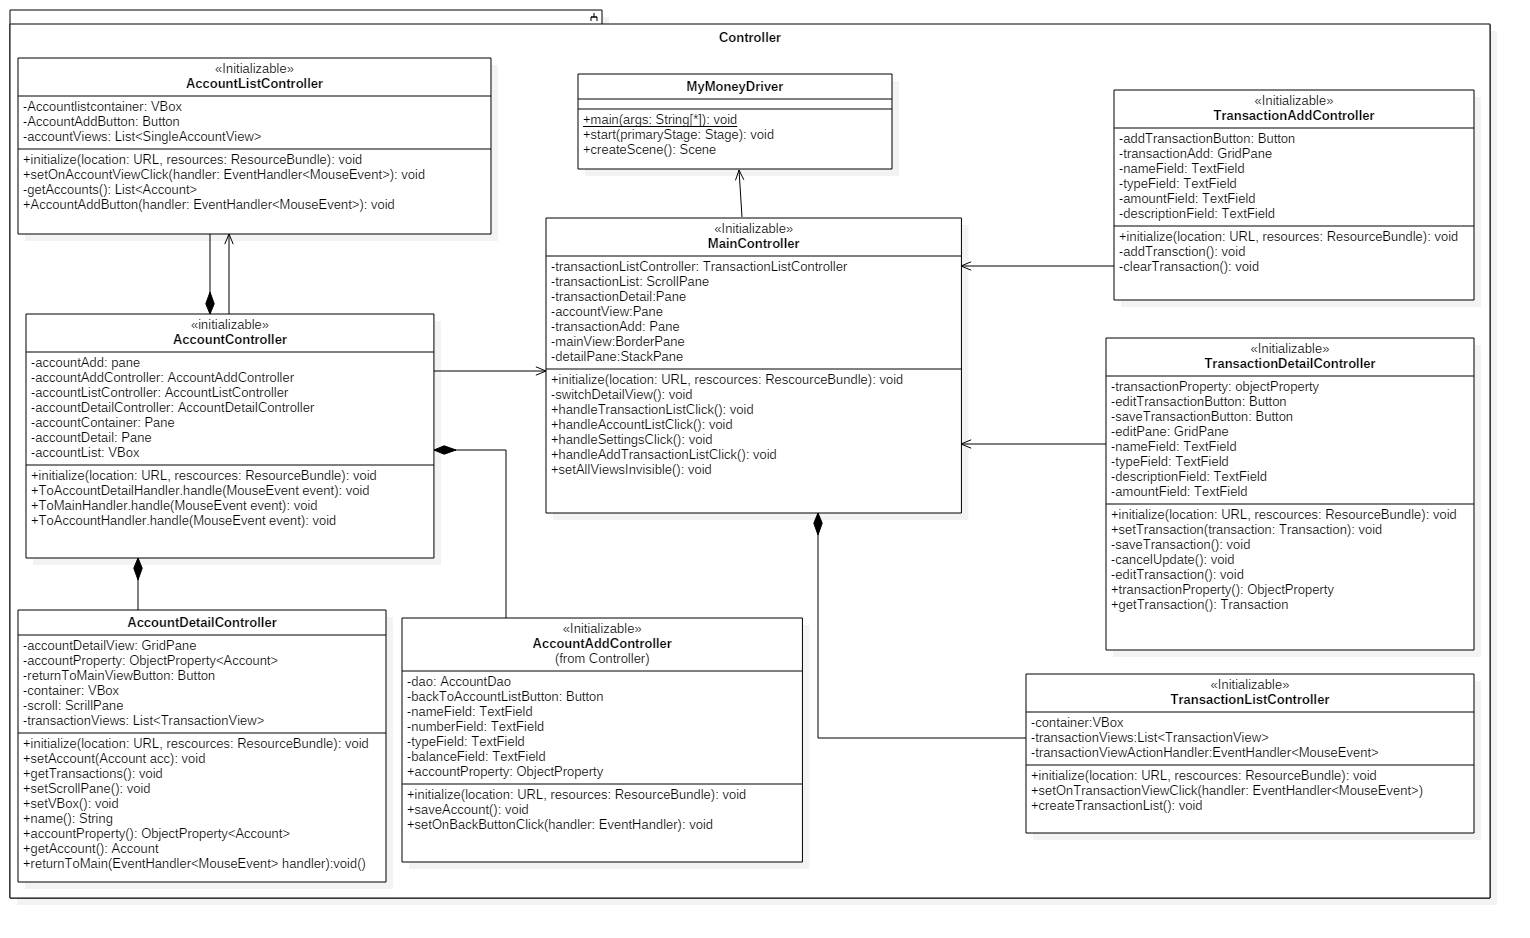
\includegraphics[width=\graphicwidth]{images/Controller.png}
\captionof{figure}{Controller Module Class Diagram}
\subsubsection{Units Description}
Controller classes and methods use the model's 'Data Access Objects' to retrieve information from the database and store it in the respective model classes(Transaction, Type Account) to be placed into the dynamic elements of the view .fxml files. Controllers also set visibility and invisibility of views.
\paragraph{Class MyMoneyDriver}
\begin{table}[H]
	\begin{tabular}{|a|p{15cm}|}
		\hline
		\rowcolor{LightCyan}
		{Class Name} & {MyMoneyDriver} \\
		\hline
		Description & The starter code for the application using Java's main function\\
		\hline
		Methods & 		 
		\begin{tabular}{| p{2cm} | p{5cm} | p{6.9cm} |}
			\hline
			\rowcolor{gray}
			{Visibility} &{Name} & {Description} \\
			\hline
			\rowcolor{white}			
			public static & main(args: String[*])  & begins the program\\
			\hline
			public & start(primaryStages:Stage)  & Sets the window properties and drives the controllers to create application \\
			\hline
			public & createScene() & Sets up the MainView.fxml class and CSS\\
			\hline			
		\end{tabular}								 
	\end{tabular}
\end{table}

\paragraph{MyMoneyDriver Methods:}

\begin{tabular}{ |p{3cm}||p{\colWidth}|  }
	\hline
	Method Name &  main(args: String[*]) \\
	\hline
	Class Name & MyMoneyDriver\\
	\hline
	Functionality & Begins the application\\
	\hline
	Input & start fields\\
	\hline
	Output & -\\
	\hline
	Pseudo Code&BEGIN\\ & launch javafx environment\\&END\\
	\hline
\end{tabular}  

\begin{tabular}{ |p{3cm}||p{\colWidth}|  }
	\hline
	Method Name &  start(primaryStages:Stage) \\
	\hline
	Class Name & MyMoneyDriver\\
	\hline
	Functionality & Sets up the JavaFX window properties\\
	\hline
	Input & Window to be used\\
	\hline
	Output & -\\
	\hline
	Pseudo Code & BEGIN \\
	& 	primaryStage.setTitle("MyMoney Application");\\
	& 	primaryStage.setScene(createScene());\\
	& primaryStage.setResizable(false);\\
	& primaryStage.show();\\
	& END\\
	\hline
\end{tabular}  

\begin{tabular}{ |p{3cm}||p{\colWidth}|  }
	\hline
	Method Name &  createScene() \\
	\hline
	Class Name & MyMoneyDriver\\
	\hline
	Functionality & Creates the mainview window and stylesheet\\
	\hline
	Input & -\\
	\hline
	Output & -\\
	\hline
	Pseudo Code & BEGIN \\
	& Load the mainview.fxml with FXMLLoader and add stylesheet.\\
	& Set view size\\
	& END \\
	\hline
\end{tabular}  

\paragraph{Class MainController}
\begin{table}[H]
	\begin{tabular}{|a|p{15cm}|}
		\hline
		\rowcolor{LightCyan}
		{Class Name} & {MainController} \\
		\hline
		Description & The main controller controls the MainView fxml files and coordinates which display should be used from the main.\\
		\hline
		Attributes & 
		\begin{tabular}{| p{1.5cm} | p{4.5cm} | p{4.45cm} | p{3.0cm} |}
			\hline
			\rowcolor{lightgray}
			Visibility & Data Type & Name & Description \\
			\rowcolor{white}
			\hline
			private & TransactionListController & transactionListController & A reference to a transactionListController\\
			\hline
			private & ScrollPane & transactionList & Scrollplane that gets filled with TransactionView objects  \\
			\hline
			private & Pane & transactionDetail & Holds information on transactions.  \\
			\hline
			private & Pane & accountView & A view object of accounts to be controlled \\
			\hline
			private & Pane & transactionAdd & A view object of Transactions to be controlled. Deals with transaction creation. \\
			\hline
			private & BorderPane & mainView & A view object of Main to be controlled \\
			\hline
			private & StackPane & detailPane & A view object of Main to be controlled \\
			\hline
		\end{tabular} \\
		\hline
		Methods & 		 
		\begin{tabular}{| p{1.5cm} | p{6.5cm} | p{5.9cm} |}
			\hline
			\rowcolor{gray}
			{Visibility} &{Name} & {Description} \\
			\hline
			\rowcolor{white}			
			public & initialize(location:URL, rescources:RescourceBundle) & provides class with necessary controller info\\
			\hline
			private&  switchDetailView() & Transfers the current seen object to detailview \\
			\hline
			public 	& handleTransactionListClick()  & Use the transaction list controller to shift views\\
			\hline
			public 	& handleAccountListClick() & Use the account list controller to shift views\\
			\hline
			public 	&  handleSettingsClick() & Shift views to settings\\
			\hline
			public &  handleAddTransactionListClick() & Switch views add transaction list through it's controller\\
			\hline
			public & setAllViewsInvisible()  & Set all panes to invisible with their controllers\\
			\hline
			
		\end{tabular}								 
	\end{tabular}
\end{table}

\paragraph{MainController Methods:}
\begin{tabular}{ |p{3cm}||p{\colWidth}|  }
	\hline
	Method Name &  initialize(location:URL, rescources:RescourceBundle) \\
	\hline
	Class Name & MainController\\
	\hline
	Functionality & Sets all views invisible, sets account view visible and then sets up transactionListController to handle events\\
	\hline
	Input & Database URL and view resource\\
	\hline
	Output & -\\
	\hline
	Pseudo Code & BEGIN\\
	& setAllViewsInvisible() \\
	& accountView.setVisible(true) \\
	& transactionListController.setOnTransactionViewClick(new TransactionViewClickHandler()) \\
	& END\\
	\hline
\end{tabular}  

\begin{tabular}{ |p{3cm}||p{\colWidth}|  }
	\hline
	Method Name &  switchDetailView() \\
	\hline
	Class Name & MainController\\
	\hline
	Functionality & Flips the views over from list to detail\\
	\hline
	Input &-\\
	\hline
	Output & -\\
	\hline
	Pseudo Code & BEGIN\\
	& transactionList.setVisible(NOT transactionList.isVisible()) \\
	& transactionDetail.setVisible(NOT transactionDetail.isVisible()) \\
	& END\\
	\hline
\end{tabular}

\begin{tabular}{ |p{3cm}||p{\colWidth}|  }
	\hline
	Method Name &  handleTransactionListClick() \\
	\hline
	Class Name & MainController\\
	\hline
	Functionality & Switches view to transaction detail view and builds it's list\\
	\hline
	Input &-\\
	\hline
	Output & -\\
	\hline
	Pseudo Code & BEGIN\\
	&	transactionListController.createTransactionList() \\
	&	setAllViewsInvisible() \\
	&	transactionList.setVisible(true) \\
	& END\\
	\hline
\end{tabular}    

\begin{tabular}{ |p{3cm}||p{\colWidth}|  }
	\hline
	Method Name &  handleAccountListClick() \\
	\hline
	Class Name & MainController\\
	\hline
	Functionality & Switches view to account detail view\\
	\hline
	Input &-\\
	\hline
	Output & -\\
	\hline
	Pseudo Code & BEGIN\\
	& setAllViewsInvisible();\\
	& accountView.setVisible(true);\\
	& END\\
	\hline
\end{tabular}    

\begin{tabular}{ |p{3cm}||p{\colWidth}|  }
	\hline
	Method Name &  handleAddTransactionClick() \\
	\hline
	Class Name & MainController\\
	\hline
	Functionality & Switches view to add transaction detail view\\
	\hline
	Input &-\\
	\hline
	Output & -\\
	\hline
	Pseudo Code & BEGIN\\
	&		setAllViewsInvisible();\\
	& 		transactionAdd.setVisible(true);\\
	& END\\
	\hline
\end{tabular}   

\begin{tabular}{ |p{3cm}||p{\colWidth}|  }
	\hline
	Method Name &  setAllViewsInvisible() \\
	\hline
	Class Name & MainController\\
	\hline
	Functionality & Switches all views to invisible\\
	\hline
	Input &-\\
	\hline
	Output & -\\
	\hline
	Pseudo Code & BEGIN\\
	&	transactionAdd.setVisible(false); \\
	&	accountView.setVisible(false);\\
	&	transactionList.setVisible(false);\\
	&	transactionDetail.setVisible(false);\\
	&	statisticsView.setVisible(false);\\
	& END\\
	\hline
\end{tabular}   

\paragraph{Class TransactionAddController}
\begin{table}[H]
	\begin{tabular}{|a|p{15cm}|}
		\hline
		\rowcolor{LightCyan}
		{Class Name} & {TransactionAddController} \\
		\hline
		Description & The TransactionAddController is the controller object for the TransactionAdd.fxml file for adding transactions. It's methods relate to the manipulation of view items on this scene.\\
		\hline
		Attributes & 
		\begin{tabular}{| p{1.5cm} | p{2.5cm} | p{4.45cm} | p{5.0cm} |}
			\hline
			\rowcolor{lightgray}
			Visibility & Data Type & Name & Description \\
			\rowcolor{white}
			\hline
			private & Button & addTransactionButton & Button is pressed to confirm the addition of  a new transaction\\
			\hline
			private & GridPane & transactionAdd & Form container for transaction add data\\
			\hline
			private & TextField & nameField & New transaction field data\\
			\hline
			private & TextField & typeField & New transaction field data\\
			\hline
			private & TextField & amountfield & New transaction field data\\
			\hline
			private & TextField & descriptionField & New transaction field data\\
			\hline	
		\end{tabular} \\
		\hline
		Methods & 		 
		\begin{tabular}{| p{1.5cm} | p{6.5cm} | p{5.9cm} |}
			\hline
			\rowcolor{gray}
			{Visibility} &{Name} & {Description} \\
			\hline
			\rowcolor{white}			
			public &  initialize(location:URL, resources: ResourceBundle) & Initializes the controller and creates connection to database\\
			\hline
			public &  addTransction() & Communicate with the server to send field data to the server\\
			\hline
			public &  clearTransaction() & Set all the data fields to blank\\
			\hline			
		\end{tabular}								 
	\end{tabular}
\end{table}

\paragraph{TransactionAddController Methods:}
\begin{tabular}{ |p{3cm}||p{\colWidth}|  }
	\hline
	Method Name &  initialize(location:URL, rescources:RescourceBundle) \\
	\hline
	Class Name & TransactionAddController\\
	\hline
	Functionality & Sets up a connection to the Dao and Database then fills out data fields with items\\
	\hline
	Input & Database URL and view resource\\
	\hline
	Output & -\\
	\hline
	Pseudo Code & BEGIN\\
	& 		AccountDao dbAccount=new AccountDao() \\
	& 	for (Account e: dbAccount.getAllAccounts()) \\
	&		comboBox.getItems().add(e.getId()+". "+e.getName()) \\
	& END\\
	\hline
\end{tabular}  

\begin{tabular}{ |p{3cm}||p{\colWidth}|  }
	\hline
	Method Name &  addTransaction() \\
	\hline
	Class Name & TransactionAddController\\
	\hline
	Functionality & Reads fields and sends the data to the Database for saving through the DAO after formating\\
	\hline
	Input & - \\
	\hline
	Output & -\\
	\hline
	Pseudo Code & BEGIN\\
	& 	transDAO = new TransactionDao() \\
	& 	typeDao = new TypeDao \\
	&	*GET DATA FIELDS \\
	& 	t = new Transaction(*DATA FIELDS)\\
	& 	transDAO.insert(t)\\
	& clearTransaction()\\
	& END\\
	\hline
\end{tabular} 

\begin{tabular}{ |p{3cm}||p{\colWidth}|  }
	\hline
	Method Name &  clearTransaction() \\
	\hline
	Class Name & TransactionAddController\\
	\hline
	Functionality & Set all data fields to blank\\
	\hline
	Input & -\\
	\hline
	Output & -\\
	\hline
	Pseudo Code & BEGIN\\
	& 	*SET ALL DATA FIELDS TO "" \\&END\\
	\hline
\end{tabular} 

\paragraph{Class TransactionDetailController}
\begin{table}[H]
	\begin{tabular}{|a|p{15cm}|}
		\hline
		\rowcolor{LightCyan}
		{Class Name} & {TransactionDetailController} \\
		\hline
		Description & The TransactionDetailController is the controller object for the TransactionDetail.fxml file for viewing specifics about transactions. It's methods relate to the manipulation of view items on this scene.\\
		\hline
		Attributes & 
		\begin{tabular}{| p{1.5cm} | p{2.5cm} | p{4.45cm} | p{5.0cm} |}
			\hline
			\rowcolor{lightgray}
			Visibility & Data Type & Name & Description \\
			\rowcolor{white}
			\hline
			private & objectProperty $\langle Transaction \rangle$ & transactionProperty & Extended Transaction class with ObjectProperty methods \\
			\hline
			private & Button & editTransactionButton & Button to trigger the editing pane \\
			\hline
			private & Button & saveTransactionButton & Button to trigger the saving pane\\
			\hline
			private & TextField & editField & Form field for editing\\
			\hline
			private & TextField & nameField & Form field for editing\\
			\hline
			private & TextField & descriptionField & Form field for editing\\		
			\hline
			private & TextField & amountField & Form field for editing\\		
			\hline
		\end{tabular} \\
		\hline
		Methods & 		 
		\begin{tabular}{| p{1.5cm} | p{6.5cm} | p{5.9cm} |}
			\hline
			\rowcolor{gray}
			{Visibility} &{Name} & {Description} \\
			\hline
			\rowcolor{white}			
			public &  initialize(location:URL, resources:ResourceBundle) & Open connection to the database \\
			\hline
			public &  setTransaction(transaction: Transaction) & Set transactionProperty to argument\\
			\hline
			private &  saveTransaction() & send transaction to database from form fields\\
			\hline
			private &  cancelTransaction() & Go back to the detailPane[TransactionDetailControler]\\			
			\hline
			private &  editTransaction() & Open edit pane and fill out forms with the transaction called to be edited\\		
			\hline
			public &  transactionProperty() & returns transactionProperty\\		
			\hline
			public &  getTransaction() & returns the transaction linked to transactionProperty\\
			\hline			
		\end{tabular}								 
	\end{tabular}
\end{table}

\paragraph{TransactionDetailController Methods:}

\begin{tabular}{ |p{3cm}||p{\colWidth}|  }
	\hline
	Method Name &  initialize(location:URL, rescources:RescourceBundle) \\
	\hline
	Class Name & TransactionDetailController\\
	\hline
	Functionality & Sets up a connection to the Dao and Database then fills out data fields with items\\
	\hline
	Input & Database URL and view resource\\
	\hline
	Output & -\\
	\hline
	Pseudo Code & BEGIN\\
	& 		AccountDao dbAccount=new AccountDao() \\
	& 	for (Account e: dbAccount.getAllAccounts()) \\
	&		comboBox.getItems().add(e.getId()+". "+e.getName()) \\
	& END\\
	\hline
\end{tabular}  

\begin{tabular}{ |p{3cm}||p{\colWidth}|  }
	\hline
	Method Name &  setTransaction(transaction: Transaction) \\
	\hline
	Class Name & TransactionDetailController\\
	\hline
	Functionality & Sets the transactionProperty to transaction and makes detailPane visible\\
	\hline
	Input & Transaction to set as the ObjectProperty\\
	\hline
	Output & -\\
	\hline
	Pseudo Code 
	& BEGIN\\
	& 		Create TransactionDao \\
	& 		Create TypeDao\\
	&		Transaction t = transactionProperty.get() \\
	& 		Get Data from fields and place it into the Transaction t. \\
	& 		Insert into database if it's a new piece of data. Otherwise update records. \\
	& 		If record of Transaction no longer has any fields (size < 1) delete it from the records. \\
	& 		Set current Pane invisible and make detail Pane visible \\
	& END\\
	\hline
\end{tabular}  

\begin{tabular}{ |p{3cm}||p{\colWidth}|  }
	\hline
	Method Name &  cancelUpdate() \\
	\hline
	Class Name & TransactionDetailController\\
	\hline
	Functionality & Make detailPane visible and editPane invisible\\
	\hline
	Input & -\\
	\hline
	Output & -\\
	\hline
	Pseudo Code & BEGIN\\
	& 	editPane.setVisible(false) \\
	& 	detailPane.setVisible(true)\\
	& END\\
	\hline
\end{tabular}  

\begin{tabular}{ |p{3cm}||p{\colWidth}|  }
	\hline
	Method Name &  editTransaction() \\
	\hline
	Class Name & TransactionDetailController\\
	\hline
	Functionality & Make detailPane invisible and editPane visible then set the TextField values to those of the Transaction object\\
	\hline
	Input & -\\
	\hline
	Output & -\\
	\hline
	Pseudo Code & BEGIN\\
	& 	editPane.setVisible(true) \\
	& 	detailPane.setVisible(false)\\
	&   get transaction from transactionProperty\\
	& 	Set each textfield field to transaction values \\ 
	& END\\
	\hline
\end{tabular}  

\begin{tabular}{ |p{3cm}||p{\colWidth}|  }
	\hline
	Method Name &  transactionProperty() \\
	\hline
	Class Name & TransactionDetailController\\
	\hline
	Functionality & Return the transaction property\\
	\hline
	Input & -\\
	\hline
	Output & ObjectProperty<Transaction>\\
	\hline
\end{tabular}  

\begin{tabular}{ |p{3cm}||p{\colWidth}|  }
	\hline
	Method Name &  getTransaction() \\
	\hline
	Class Name & TransactionDetailController\\
	\hline
	Functionality & Return the transaction from the transaction property\\
	\hline
	Input & -\\
	\hline
	Output & Transaction\\
	\hline
\end{tabular}  







\paragraph{Class TransactionListController}
\begin{table}[H]
	\begin{tabular}{|a|p{15cm}|}
		\hline
		\rowcolor{LightCyan}
		{Class Name} & {TransactionListController} \\
		\hline
		Description & The TransactionListController is the controller object for the TransactionList.fxml file. It's methods relate to the manipulation of view items on this scene as well as produce additonal view objects inside of the TransactionList.fxml scene such as the TransactionView.\\
		\hline
		Attributes & 
		\begin{tabular}{| p{1.5cm} | p{5cm} | p{3.5cm} | p{3.45cm} |}
			\hline
			\rowcolor{lightgray}
			Visibility & Data Type & Name & Description \\
			\hline
			\rowcolor{white}
			private & VBox & container & A container object for holding TransactionView objects\\ 
			\hline
			private & VBox & containerType & A container object for holding TransactionView objects sorted by type\\ 
			\hline
			private & List$\langle TransactionView \rangle$ & transactionViews & A List of transactionView Objects to be placed in VBox\\
			\hline
			private & List$\langle TransactionView \rangle$ & transactionViewsByType & A List of transactionView Objects by type to be placed in a VBox\\
			\hline
			private & EventHandler$\langle MouseEvent \rangle$  & transactionViewActionHandler & A handler for click events on given view objects\\		
			\hline	
		\end{tabular} \\
		\hline
		Methods & 		 
		\begin{tabular}{| p{2cm} | p{5cm} | p{6.9cm} |}
			\hline
			\rowcolor{gray}
			{Visibility} &{Name} & {Description} \\
			\hline
			\rowcolor{white}			
			public &  initialize(in location:URL, in resources:ResourceBundle) & Generate the two initial transaction view array lists\\
			\hline
			public & setOnTransactionViewClick(EventHandler<MouseEvent> handler) & set the basic TransactionView click handler\\
			\hline
			public & createTransactionList() & clears previous settings, opens a connection to the database through the dao and creates all TransactionViews from database data. \\
			\hline
			public &  getTransactions() & uses the TransactionDao to retrieve all transactions from the database in a list\\
			\hline			
		\end{tabular}								 
	\end{tabular}
\end{table}

\paragraph{TransactionListController Methods: }

\begin{tabular}{ |p{3cm}||p{\colWidth}|  }
	\hline
	Method Name &  initialize(location:URL, rescources:RescourceBundle) \\
	\hline
	Class Name & TransactionListController\\
	\hline
	Functionality & Creates two new arraylists for containing TransactionViews\\
	\hline
	Input & Database URL and view resource\\
	\hline
	Output & -\\
	\hline
	Pseudo Code & BEGIN\\
	& Generate 2 new TransactionView ArrayLists \\
	& END\\
	\hline
\end{tabular} 

\begin{tabular}{ |p{3cm}||p{\colWidth}|  }
	\hline
	Method Name & setOnTransactionViewClick(EventHandler<MouseEvent> handler) \\
	\hline
	Class Name & TransactionListController\\
	\hline
	Functionality & Sets the event handler for TransactionView click events\\
	\hline
	Input & The handler to be assigned\\
	\hline
	Output & -\\
	\hline
	Pseudo Code & BEGIN\\
	& transactionViewActionHandler = handler\\
	& END\\
	\hline
\end{tabular} 

\begin{tabular}{ |p{3cm}||p{\colWidth}|  }
	\hline
	Method Name & createTransactionList()\\
	\hline
	Class Name & TransactionListController\\
	\hline
	Functionality & Clears both of the Array lists and their respective VBoxes, opens connection to the Dao and creates a set of TransactionView objects from all Transactions and Types stored on the database. It then assigns all Transaction and Type View records into each container after assigning them an event handler. \\
	\hline
	Input & -\\
	\hline
	Output & -\\
	\hline
	Pseudo Code & BEGIN\\
	& Clear both transactionView ArrayLists\\
	& Clear both VBox contents\\
	& Open connection to database \\
	& Retrieve all transactions and types \\
	& For all data in array lists assign them the click event handler \\
	& Assign all data to their respective VBoxes \\
	& END\\
	\hline
\end{tabular} 

\begin{tabular}{ |p{3cm}||p{\colWidth}|  }
	\hline
	Method Name & getTransactions()\\
	\hline
	Class Name & TransactionListController\\
	\hline
	Functionality & Creates a TransactionDao connection to the database and then retrieves all of the database's transactions \\
	\hline
	Input & -\\
	\hline
	Output & List $\langle Transaction \rangle$\\
	\hline
	Pseudo Code & BEGIN\\
	& 		TransactionDao transactionDao = new TransactionDao();\\
	& 		return transactionDao.getAllTransactions(); \\
	& END\\
	\hline
\end{tabular} 

\paragraph{Class AccountListController}
\begin{table}[H]
	\begin{tabular}{|a|p{15cm}|}
		\hline
		\rowcolor{LightCyan}
		{Class Name} & {AccountListController} \\
		\hline
		Description & The AccountListController controls AccountList.fxml to fill a VBox container with a list of all accounts in the database and interactions with generated SingleAcountView objects it generates.\\
		\hline
		Attributes & 
		\begin{tabular}{| p{1.5cm} | p{5cm} | p{3.5cm} | p{3.45cm} |}
			\hline
			\rowcolor{lightgray}
			Visibility & Data Type & Name & Description \\
			\hline
			\rowcolor{white}
			private & Button & NewAccountButton & A button to be pressed to trigger new accounts being added to the database.\\
			\hline
			private & VBox & accountListContainer & The location where SingleAccountView objects will be stored\\
			\hline
			private & List$\langle SingleAccountView \rangle$  & accountViews & A List of all accounts to be placed into the VBox\\	
			\hline	
			private & AccountController & accountController & Reference to the AccountController object this object is contained in\\
			\hline
			private&  EventHandler $\langle MouseEvent \rangle$ & accountViewActionHandler& The handler that will activate on account view clicks\\
			\hline
			private &Button & returnToMainViewButton & Button to return user back to main view\\
			\hline
		\end{tabular} \\
		\hline
		Methods & 		 
		\begin{tabular}{| p{2cm} | p{5cm} | p{6.9cm} |}
			\hline
			\rowcolor{gray}
			{Visibility} &{Name} & {Description} \\
			\hline
			\rowcolor{white}			
			public &  initialize(location:URL, resources:ResourceBundle) & Initializes the acountViews arraylist\\
			\hline
			public &  setupAccounts(EventHandler<MouseEvent> handler) &  Assigns the handler field to argument and array list variables, clears vboxes and adds SingleAccountViews to them\\
			\hline
			private &  getAccounts() & creates an AccountDao then retrieves and returns all Accounts in the database\\
			\hline		
			public &  AccountAddClick(handler:EventHandlerList$\langle MouseEvent \rangle$) & Assigns an event handler to the NewAccountButton\\
			\hline	
		\end{tabular}								 
	\end{tabular}
\end{table}

\paragraph{AccountListController Methods:}

\begin{tabular}{ |p{3cm}||p{\colWidth}|  }
	\hline
	Method Name &  initialize(location:URL, rescources:RescourceBundle) \\
	\hline
	Class Name & AccountListController\\
	\hline
	Functionality & Creates a new arraylist for containing AccountViews\\
	\hline
	Input & Database URL and view resource\\
	\hline
	Output & -\\
	\hline
	Pseudo Code & BEGIN\\
	& Generate a new SingleAccountView ArrayList \\
	& END\\
	\hline
\end{tabular} 


\begin{tabular}{ |p{3cm}||p{\colWidth}|  }
	\hline
	Method Name & setupAccounts(EventHandler$\langle MouseEvent \rangle$)\\
	\hline
	Class Name & AccountListController\\
	\hline
	Functionality & Sets the SingleAccountView click handler, clears the ArrayList for each accountViews and the VBox, then retrieves all accounts, creates SingleAccountView items, places them in the container and adds event handlers to each of them. \\
	\hline
	Input & EventHandler to be triggered on any SingleAccountView click\\
	\hline
	Output & -\\
	\hline
	Pseudo Code & BEGIN\\
	& Assign handler\\
	& Clear ArrayList\\
	& Clear VBox contents\\
	& Get all accounts from database\\
	& Create them and assign them their handler\\
	& Add them to the VBox \\
	& END\\
	\hline
\end{tabular} 

\begin{tabular}{ |p{3cm}||p{\colWidth}|  }
	\hline
	Method Name & AccountAddClick(handler:EventHandlerList$\langle MouseEvent \rangle$)\\
	\hline
	Class Name & AccountListController\\
	\hline
	Functionality & Sets the event handler for the add account button\\
	\hline
	Input & The handler to be assigned\\
	\hline
	Output & -\\
	\hline
	Pseudo Code & BEGIN\\
	& NewAccountButton.setOnMouseClicked(handler); \\
	& END\\
	\hline
\end{tabular} 

\begin{tabular}{ |p{3cm}||p{\colWidth}|  }
	\hline
	Method Name & getAccounts()\\
	\hline
	Class Name & AccountListController\\
	\hline
	Functionality & Creates an AccountDao connection to the database and then retrieves all of the database's accounts \\
	\hline
	Input & -\\
	\hline
	Output & List $\langle Account \rangle$\\
	\hline
	Pseudo Code & BEGIN\\
	& 		AccountDao AccountDao = new AccountDao();\\
	& 		return accountDao.getAllAccounts(); \\
	& END\\
	\hline
\end{tabular} 



\paragraph{Class AccountController}
\begin{table}[H]
	\begin{tabular}{|a|p{15cm}|}
		\hline
		\rowcolor{LightCyan}
		{Class Name} & {AccountController} \\
		\hline
		Description & The AccountController class controls AccountView.fxml in order to display the view the user wants to see. It contains the controllers for AccountAddController, AccountListController and AccountDetailController in order to respond to user requests to view certain Views\\
		\hline
		Attributes & 
		\begin{tabular}{| p{1.5cm} | p{4.4cm} | p{4.1cm} | p{3.45cm} |}
			\hline
			\rowcolor{lightgray}
			Visibility & Data Type & Name & Description \\
			\rowcolor{white}
			\hline
			private &  Pane & accountAdd & The pane to hold AccountAdd views\\
			\hline
			private& AccountAddController& accountAddController& The controller of AccountAdd views\\
			\hline
			private& AccountListController& accountListController& The controller of AccountList views\\
			\hline
			private &AccountDetailController &accountDetailController&The controller of AccountDetail views\\
			\hline
			private& Pane &accountContainer&The pane to hold AccountList views\\
			\hline
			private &Pane& accountDetail& The pane to hold AccountDetail views\\
			\hline
			private & VBox & accountList & The container to store a list of accounts\\
			\hline
		\end{tabular} \\
		\hline
		Methods & 		 
		\begin{tabular}{| p{1.7cm} | p{7.0cm} | p{5.2cm} |}
			\hline
			\rowcolor{gray}
			{Visibility} &{Name} & {Description} \\
			\hline
			\rowcolor{white}			
			public &  initialize(location: URL, resources: ResourceBundle) & Initialize by setting accountList pane to visible and attaching eventHandlers to each controllers navigation buttons\\
			\hline
			public &  ToAccountDetailHandler.handle (MouseEvent event) & Switches views to the AccountDetail.fxml view\\
			\hline
			public &  ToMainHandler.handle (MouseEvent event) & Switches views to the MainView.fxml view\\
			\hline			
			public& ToAccountHandler.handle (MouseEvent event) & Switches to the AccountAdd.fxml View \\
			\hline
		\end{tabular}								 
	\end{tabular}
\end{table}

\paragraph{AccountController Methods:}


\begin{tabular}{ |p{3cm}||p{\colWidth}|  }
	\hline
	Method Name &  initialize(location:URL, rescources:RescourceBundle) \\
	\hline
	Class Name & AccountController\\
	\hline
	Functionality & Sets all views to invisible except the AccountList view the adds event handlers to each controller's navigation buttons\\
	\hline
	Input & Database URL and view resource\\
	\hline
	Output & -\\
	\hline
	Pseudo Code & BEGIN\\
	&	1. Set visibility all to false, except account list \\
	& 	2. Assign event handlers to each controller's navigation buttons using ToAccountDetailHandler.handle(MouseEvent event), ToMainHandler.handle(MouseEvent event) and ToAccountHandler.handle(MouseEvent event) \\
	& END\\
	\hline
\end{tabular} 


\begin{tabular}{ |p{3cm}||p{\colWidth}|  }
	\hline
	Method Name & ToAccountDetailHandler.handle(MouseEvent event)\\
	\hline
	Class Name & AccountController\\
	\hline
	Functionality & Sets up the Accounts contained in the AccountDetailController then sets the AccountDetail view to be visible and all others to be invisible\\
	\hline
	Input & The event being fired on the handler\\
	\hline
	Output & -\\
	\hline
	Pseudo Code & BEGIN\\
	& Create SingleAccountView from event source\\
	& Gets Account from the SingleAccountView\\
	& Sets the accountDetailController's account to the Account\\
	& Set all panes invisible except AccountDetail \\
	& END\\
	\hline
\end{tabular} 

\begin{tabular}{ |p{3cm}||p{\colWidth}|  }
	\hline
	Method Name & ToMainHandler.handle(MouseEvent event)\\
	\hline
	Class Name & AccountController\\
	\hline
	Functionality & Sets all panes to be invisible except from AccountList\\
	\hline
	Input & The event being fired on the handler\\
	\hline
	Output & -\\
	\hline
	Pseudo Code & BEGIN\\
	& Set all panes invisible except AccountList \\
	& END\\
	\hline
\end{tabular} 

\begin{tabular}{ |p{3cm}||p{\colWidth}|  }
	\hline
	Method Name & ToAccountAddHandler.handle(MouseEvent event)\\
	\hline
	Class Name & AccountController\\
	\hline
	Functionality & Sets all panes to be invisible except from AccountAdd\\
	\hline
	Input & The event being fired on the handler\\
	\hline
	Output & -\\
	\hline
	Pseudo Code & BEGIN\\
	& Set all panes invisible except AccountAdd \\
	& END \\
	\hline
\end{tabular} 


\paragraph{Class AccountAddController}
\begin{table}[H]
	\begin{tabular}{|a|p{15cm}|}
		\hline
		\rowcolor{LightCyan}
		{Class Name} & {AccountAddController} \\
		\hline
		Description & AccountAddController communicates with the database to store accounts into it's database through user manipulation of view objects.\\
		\hline
		Attributes & 
		\begin{tabular}{| p{2cm} | p{3.0cm} | p{4.0cm} | p{4.45cm} |}
			\hline
			\rowcolor{lightgray}
			Visibility & Data Type & Name & Description \\
			\hline
			\rowcolor{white}
			private & AccountDao & dao & Connection to the database for accounts \\
			\hline
			private & Button & backToAccountList- Button & Button to redirect user to account list \\
			\hline
			private & TextField & nameField & Field for account creation. \\
			\hline
			private & TextField & numberField & Field for account creation. \\
			\hline
			private & TextField & typeField & Field for account creation. \\
			\hline
			private & TextField & balanceField & Field for account creation. \\
			\hline
			public & ObjectProperty & accountProperty & Adds additional methods to a given variable \\
			\hline
		\end{tabular} \\
		\hline
		Methods & 		 
		\begin{tabular}{| p{2cm} | p{5cm} | p{6.9cm} |}
			\hline
			\rowcolor{gray}
			{Visibility} &{Name} & {Description} \\
			\hline
			\rowcolor{white}			
			public &  initialize(location:URL, resources:ResourceBundle) & Sets a connection to the database\\
			\hline
			public &  saveAccount() & Retrieve data in TextFields and send result to database\\
			\hline
			public &  setOnBackButtonClick(handler:EventHandler) & Attatch listener to button to go back\\
			\hline
		\end{tabular}								 
	\end{tabular}
\end{table}

\paragraph{AccountAddController Methods:}

\begin{tabular}{ |p{3cm}||p{\colWidth}|  }
	\hline
	Method Name &  initialize(location:URL, rescources:RescourceBundle) \\
	\hline
	Class Name & AccountAddController\\
	\hline
	Functionality & Sets up a connection to the Dao and Database\\
	\hline
	Input & Database URL and view resource\\
	\hline
	Output & -\\
	\hline
	Pseudo Code & BEGIN\\
	& 		AccountDao dbAccount=new AccountDao() \\
	& END\\
	\hline
\end{tabular} 

\begin{tabular}{ |p{3cm}||p{\colWidth}|  }
	\hline
	Method Name &  saveAccount() \\
	\hline
	Class Name & AccountAddController\\
	\hline
	Functionality & Reads fields and saves to database\\
	\hline
	Input & Database URL and view resource\\
	\hline
	Output & -\\
	\hline
	Pseudo Code & BEGIN\\
	& 		AccountDao dbAccount=new AccountDao() \\
	&		 a  = Get Account\\
	&	if (a == null) \{\\
	&		a = new Account();\\
	&		a.setCreate(new Date());\\
	&		a.setEdit(null);\\
	&		a.setArchived(null);\\
	&	\}\\
	&\\
	&	*GET VALUES FROM FIELDS\\
	&	\\
	&	a.setName(name);\\
	&	a.setBalance(balance);\\
	&	a.setNumber(number);\\
	&	a.setType(type);\\
	&	a.setTypeName(typeName);\\
	&	try \{\\
	&		if (accountProperty.get() == null) \{\\
	&			dao.insert(a);\\
	&		\} else \{\\
	&			dao.updateAccount(a);\\
	&		\}\\
	&\} catch (Exception ex) \{\\
	&\}\\
	& END\\
	\hline
\end{tabular} 

\begin{tabular}{ |p{3cm}||p{\colWidth}|  }
	\hline
	Method Name &  setOnBackButtonClick(EventHandler$\langle MouseEvent \rangle$ handler) \\
	\hline
	Class Name & AccountAddController\\
	\hline
	Functionality & Adds an event listener to the back button for clicks\\
	\hline
	Input & An event handler\\
	\hline
	Output & -\\
	\hline
	Pseudo Code 
	& BEGIN\\
	& 	backToAccountListButton.setOnMouseClicked(handler)\\
	& END\\
	\hline
\end{tabular} 


\section{Dynamic Design Scenarios}

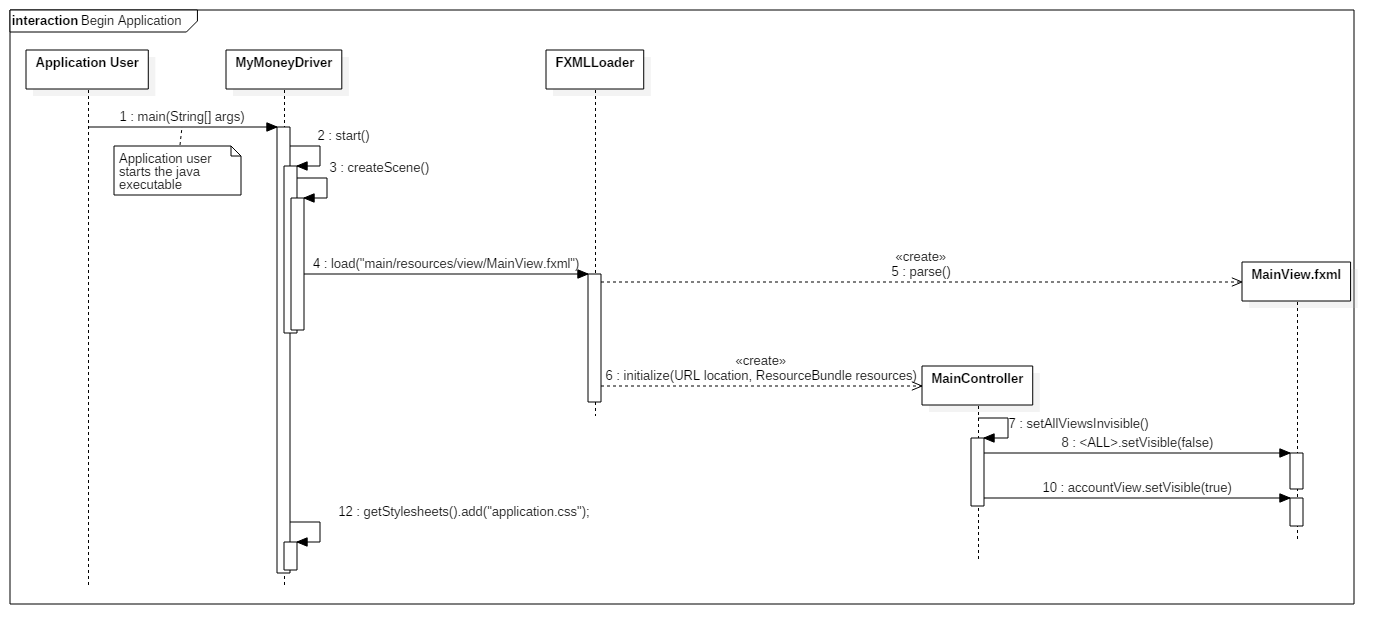
\includegraphics[width=\graphicwidth]{images/Begin_Application.png}
\captionof{figure}{Sequence Diagram of Main View Generation}

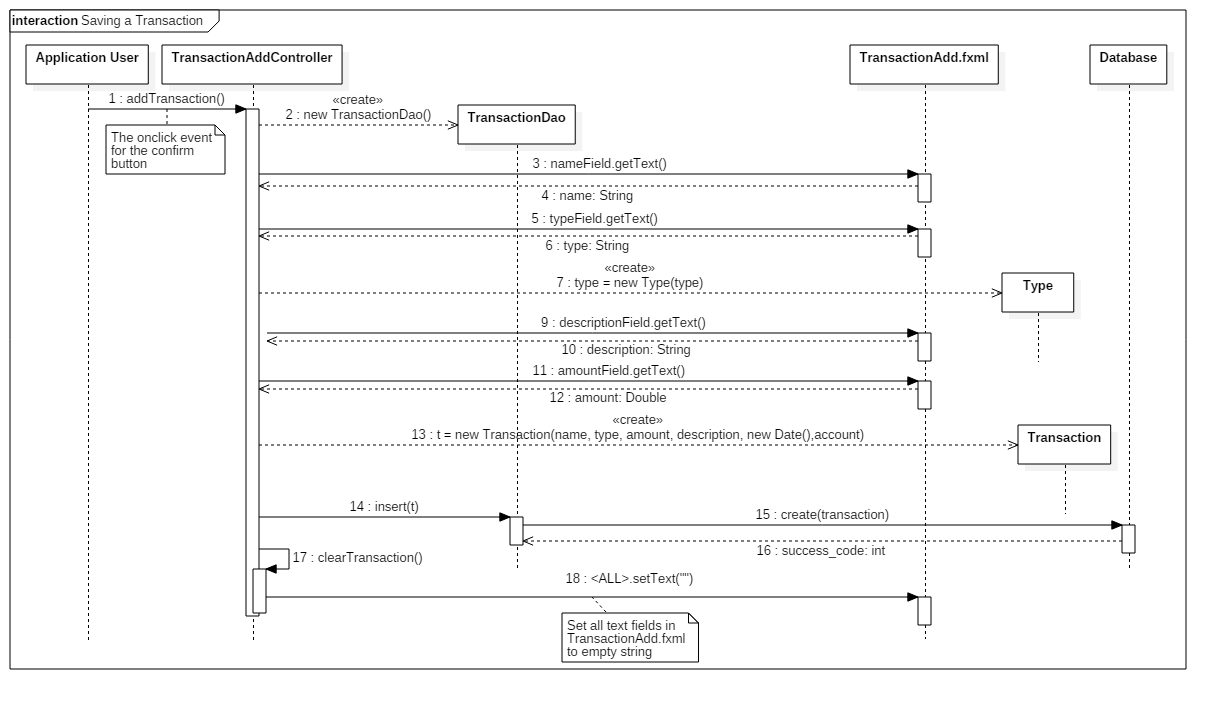
\includegraphics[width=\graphicwidth]{images/Saving_a_Transaction.png}
\captionof{figure}{Sequence Diagram of Transaction Saving}

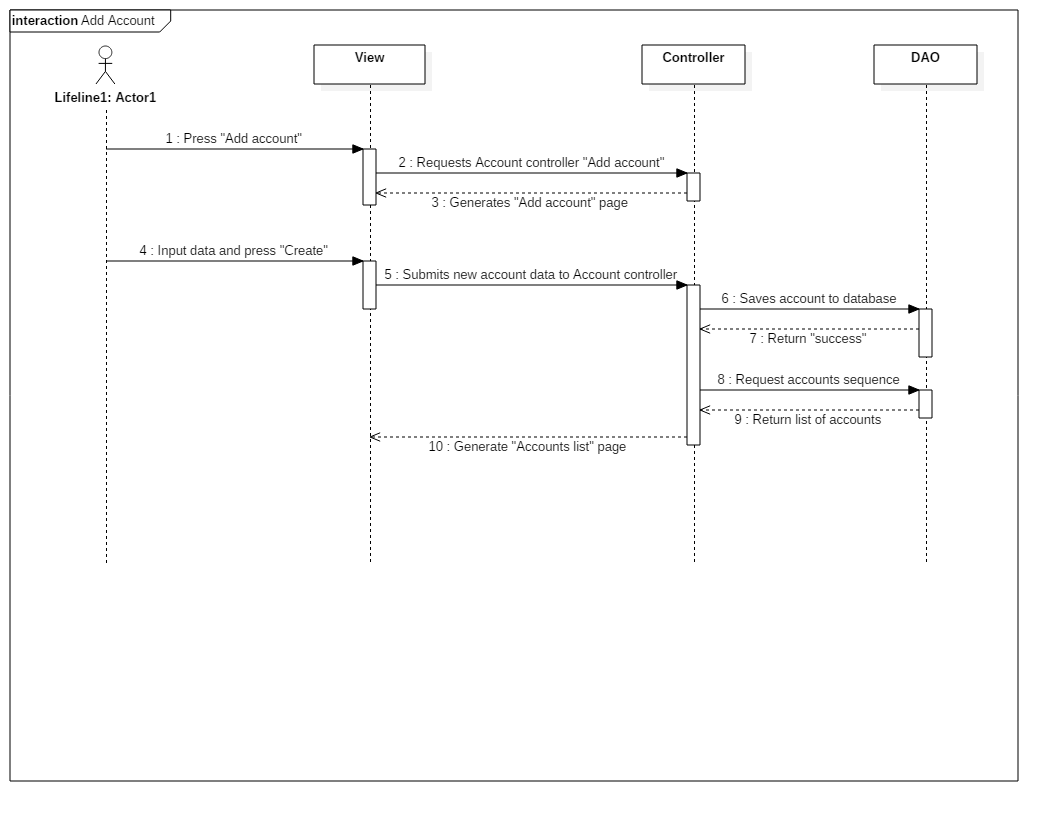
\includegraphics[width=\graphicwidth]{Add_Account}
\captionof{figure}{Sequence Diagram of Account Adding}

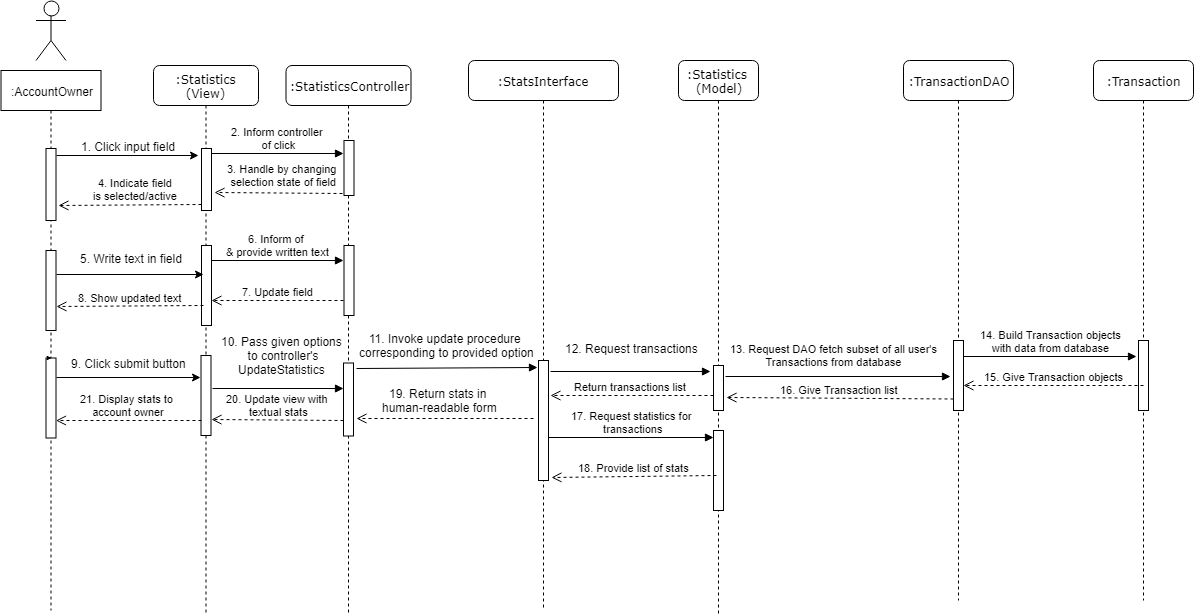
\includegraphics[width=\graphicwidth]{Statistics_Sequence}
\captionof{figure}{Sequence Diagram of Statistics System}

\section{Justification of Use-Cases and Rational}
\subsection{Drop Down Menus}
	Drop down menus are capable of conserving space in the application. By using drop downs a user can select which account he wants and which he doesn't. These dropdowns though simple in function are very practical in use.
\subsection{Statistics}
	 Statistical information is a must have on all financial applications and some users may need additional tools to conceptualize their financial situation. While the data may not be complex it is a must have to include at least a limited set of statistical functionality.
\subsection{Styling (CSS)}
	User experience is enhanced by good design. Interactions must be intuitive to the user via color, patterns, fonts and effects all drawing attention to what the user should be clicking on. Features of software should be easily discoverable and enhance the feedback given since this increases the enjoyability of using a product. Customizability is not a concern and giving the user custom control over the design does not really matter as the one design they are given is intuitive.
\subsection{Deleting Transactions}
	There must be a way to communicate with the database to remove contents that are no longer relevant. In terms of giving the user control over his or her own experience we must trust that the user knows when it's best to remove traces of his financial history from the logbooks. While there are certain dangers inherent with letting the application have the power to delete data, it's assumed that a person using financial software has the good judgment not to take excessive risks.
\subsection{View Account Transactions}
	A user will need to see his or her account transactions. Since data needs to be permanent it is necessary to put it on a database. This feature allows for users to navigate the view and click on systems to view their transaction history. Since the system already connects to the database to make insertion and delete requests, it is only natural that the user be given access to see his entire transaction table. It's assumed that the user wants to see all of the data so that freedom is given to him.
\subsection{Adding a Transaction}
	Entering in information for transaction is essential to building a database and is given four fields of data to add to a transaction. Any more data than that is deemed unnecessary for the scope of the project. Name, type, amount and description make up all the data a user can submit for a transaction since it's assumed that things like, interest rate, credit limits or anything more complicated is best left for the user to calculate himself. Also it is inherent that every transaction is marked by a unique ID number that is not set by the user himself.
\subsection{Editing an Existing Transaction}
	Users will inevitably make mistakes, when they do they will need to edit their data. It is assumed that a user can make errors on any field except for the ID therefore they are given the freedom to modify any of this data at any time from a list of all transactions they have made. Assuming they remember the name of their transaction, they can find it in a list and edit it. 
\subsection{Adding a Bank Account}
	Setting up an account is the first thing a user must do when running this software and the most fundamental. By this logic an account must be set up to use the product. Accounts are given four identification fields. Your name, your bank account number, the type of account used and the balance. Upon saving the data a table is produced in the database holding your account info. The assumption is that the user can enter any kind of bank account type he wants and edit it as he sees fit. There are more possibilities of what the user can do on the application if everything is left as a simple template he can fill out and not limit the choices that can be done by giving out radio boxes or select bars.
\subsection{Set Saving Goals}
	Since saving goals are a main reason why an individual might use a financial planning application this feature is included in the product. It is assumed that these individuals will want this goal to be fullfilled on a certain calender date. The application has textfields to fill out specifying the account balance they want to achieve by a certain date in time. Since the user is in need of keeping track of his spending against the goal, this saving's goal is presented on the account page to allow the user to constantly be reminded by it.
	
\subsection{Generate Monthly Report}
	Users will want to know how they are doing every month. A simple report displaying information on their spending, saving and frequency of use is the end goal of this product and is represented in the monthly reports. While it aims to offer a comprehensive guide of what the user has done with their money, it does not allow for multiple account views. This is due to privacy issues of people sharing computers. Finally it is important for a user to check how he is doing against his set saving goals. While no bar graphs, pie charts and histograms are generated, hopefully the user can be satisfied knowing he has met his goals and that he should continue using the software.
	

\end{document}